%%%%%%%%%%%%%%%%%%%%%%%%%%%%%%%%%%%%%%%%%%%%%%%%%%%%%%%%%%%%%%%
%
% Welcome to Overleaf --- just edit your LaTeX on the left,
% and we'll compile it for you on the right. If you open the
% 'Share' menu, you can invite other users to edit at the same
% time. See www.overleaf.com/learn for more info. Enjoy!
%
%%%%%%%%%%%%%%%%%%%%%%%%%%%%%%%%%%%%%%%%%%%%%%%%%%%%%%%%%%%%%%%
\documentclass[12pt,a4paper,oneside]{book}


\usepackage[T1]{fontenc}
\usepackage[utf8]{inputenc}
\usepackage{arabtex}
\usepackage{utf8}
\setcode{utf8}
\usepackage{babel}
\usepackage{enumitem}
\usepackage{svg}
\usepackage{amsmath}
\usepackage{amsthm}
\usepackage{amssymb}
\pdfimageresolution=150
\usepackage{tikz}
\usepackage{tcolorbox}
\usepackage{tabularx}
\usetikzlibrary{calc}
\usepackage[french,ruled,vlined]{algorithm2e}
\usepackage{rotating}
\usepackage{bbding}
\usepackage{cite}
\usepackage{lscape,graphicx}
\usepackage{rotating}
\usepackage{setspace}
\usepackage{sectsty}
\usepackage{dsfont}
\usepackage{ifpdf}
\usepackage{subfigure}
\usepackage{epsfig}
\usepackage{float}
\usepackage{titlesec}
\usepackage{multibib}
\usepackage{fancyhdr}
\usepackage{lipsum}
\usepackage{soul}
\usepackage[paperwidth=210mm,paperheight=297mm,tmargin=15mm,lmargin=20mm]{geometry}
%
\renewcommand{\topfraction}{0.9}
\renewcommand{\textfraction}{0.1}
\renewcommand{\floatpagefraction}{0.8}
%

\usepackage{hyperref}


\urlstyle{same}

\setlength{\headheight}{30pt}
\pagestyle{fancy}% \renewcommand{\chaptermark}[1]{\markboth{#1}{}}
\renewcommand{\chaptermark}[1]{\markboth{\MakeUppercase{#1}}{}}
\renewcommand{\sectionmark}[1]{\markright{\MakeUppercase{\thesection.\ #1}}}


%
% \renewcommand{\sectionmark}[1]{\markright{#1}}
%\renewcommand \thesection{\Roman{section}.}
%\renewcommand \thesubsection{\alph{subsection}.}
%
%\newcommand{\helv}{%
%\fontfamily\fontsize{9}{11}\selectfont}

%

% Clear Header Style on the Last Empty Odd pages
\makeatletter
  \def\cleardoublepage{\clearpage\if@twoside \ifodd\c@page\else%
      \hbox{}%
       \thispagestyle{empty}%              % Empty header styles
       \newpage%
       \if@twocolumn\hbox{}\newpage\fi\fi\fi}
\makeatother


\fancyhead[RE]{\textit{\nouppercase{\leftmark}}}
\fancyhead[LO]{\textit{\nouppercase{\rightmark}}}
\fancyhead[LE,RO]{\thepage}

\renewcommand{\headrulewidth}{0pt}
\renewcommand{\footrulewidth}{0pt}
%
\setcounter{secnumdepth}{4}
\setcounter{tocdepth}{4}
%

%
\def\ds{\displaystyle}
\def\dir{./figures}

%


%\setlength\topmargin{0in}
%\setlength\topmargin{0in}
%

%
% Remove page numbering from first page Bibliography
%
%%%%%%%%%%%%%%%%%%%%%%%%% Page de titre %%%%%%%%%%%%%%%%%%%%%%%
\def\baselinestretch{1.5}


\usepackage{listings}
\usepackage{caption}
\usepackage{longtable}

\usepackage{geometry}
\usepackage{booktabs}

\geometry{
    letterpaper,
    left=1.5cm,
    right=1.5cm,
    top=1.5cm,
    bottom=1.5cm
}

\usepackage{afterpage}

\newcommand\blankpage{%
    \null
    \thispagestyle{empty}%
    \addtocounter{page}{-1}%
    \newpage}


\usepackage[acronym]{glossaries}

\usepackage{lmodern}


\newenvironment{dedication}
  {%\clearpage           % we want a new page          %% I commented this
   \thispagestyle{empty}% no header and footer
   \vspace*{\stretch{1}}% some space at the top
   \itshape             % the text is in italics
   \raggedleft          % flush to the right margin
  }
  {\par % end the paragraph
   \vspace{\stretch{3}} % space at bottom is three times that at the top
   \clearpage           % finish off the page
  }


  



%\makenoidxglossaries 

%\newglossaryentry{latex}
%{
       % name=latex,
        %description={Is a mark up language specially suited for scientific documents}
%}



%\selectlanguage{English}



\hypersetup{
    colorlinks=true,
    linkcolor=black,
    filecolor=magenta,      
    urlcolor=cyan,
    pdfauthor={Name},  %put your name here
    pdftitle={PDF_TTILE},  %PDF title
    pdfpagemode=FullScreen,
    }



\begin{document}



\definecolor{codegreen}{rgb}{0,0.6,0}
    \definecolor{codegray}{rgb}{0.5,0.5,0.5}
    \definecolor{codepurple}{rgb}{0.58,0,0.82}
    \definecolor{backcolour}{rgb}{0.95,0.95,0.92}
    
    \lstdefinestyle{mystyle}{
        backgroundcolor=\color{backcolour},   
        keywordstyle=\color{magenta},
        numberstyle=\tiny\color{codegreen},
        stringstyle=\color{codepurple},
        basicstyle=\ttfamily\footnotesize,
        breakatwhitespace=false,         
        breaklines=true,                 
        captionpos=b,                    
        keepspaces=true,                 
        numbers=left,                    
        numbersep=5pt,                  
        showspaces=false,                
        showstringspaces=false,
        showtabs=false,                  
        tabsize=2
    }




%\include{Frontmatter/Page_de_garde} %FRENCH ONE

\thispagestyle{empty}
\noindent

\includegraphics[scale=0.17]{Logos/Logo_INPT.png} 
\hfill  % Automatically calculates the perfect space so it doesn't overflow horizontally

\includegraphics[scale=0.12]{Logos/Logo_ANRT.jpg}
        
\vspace{0.5cm} % Reduced slightly to save vertical space
\begin{center}
{\large \textsc{\textbf{End-of-Year Project Report (PFA)}}}\\[0.1cm]
{\large \textsc{Module: DEVELOPMENT PROJECT}}\\[0.1cm]
{\large \textsc{\textit{Major: Advanced Software Engineering for Digital Services (ASEDS)}}} \\[0.05cm] 
\vspace{-0.04cm}

% Title
\rule{\linewidth}{0.3mm} \\[0.4cm]   
 { \huge \textbf{ Design and Development of an Advanced LegalTech Platform using RAG to Answer Queries on Moroccan Law }} \\[0.15cm] 
\rule{\linewidth}{0.3mm} \\[0.4cm]
\vspace{0.2cm}


\vspace{0.6cm} 

% Authors
\noindent
\begin{minipage}{0.9\textwidth}
  \begin{flushleft} \large
    \emph{Prepared by :}\\
     Oualid \textsc{AMTOUT}   \\ Youness \textsc{ESSABRI} \\
  \end{flushleft}
\end{minipage}
\\[0.5cm]

% Supervisor
{\large \textit{Supervised by :}}\\[0.2cm]

\large Pr. Zineb \textsc{EL AKKAOUI} \hspace{0.2cm} \large (INPT)\\[0.1cm]

\vfill % <--- MAGIC COMMAND: Acts as a spring to push everything below this exactly to the bottom margin

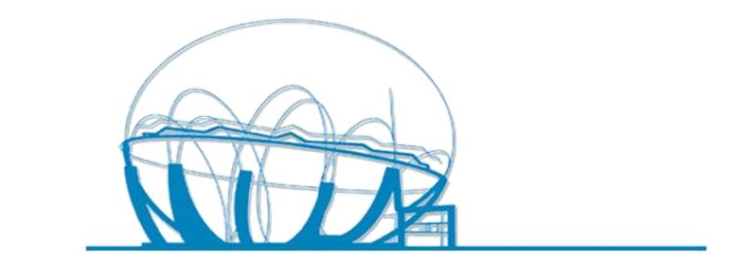
\includegraphics[scale=0.55]{Logos/ZLAFA.png} % Scaled down slightly to be safe

\vspace{0.2cm}
\textsc{Agence Nationale de Réglementation des Télécommunications}\\
\textsc{Institut National des Postes et Télécommunications}

% Bottom of the page
\vspace{0.2cm}
{\large Academic Year : 2025/2026}
   
\end{center} % ENGLISH

\afterpage{\blankpage}  %page vide obligatoire

\frontmatter


\input{Frontmatter/Dedication}


\input{Frontmatter/Acknowledgements}


\chapter*{Résumé}
\addcontentsline{toc}{chapter}{Résumé}

Avec l'évolution rapide des technologies d'Intelligence Artificielle, les modèles de langage ont prouvé une grande efficacité pour assimiler d'énormes quantités d'informations et les reformuler afin de répondre à des questions complexes. En revanche, les consultations juridiques traditionnelles et l'analyse de dossiers restent des processus très coûteux. Une utilisation appropriée de l'IA peut réduire ce coût de manière drastique pour le rendre presque symbolique.

Notre objectif à travers ce projet de fin d'année est de développer une plateforme numérique intégrée permettant aux utilisateurs d'obtenir des consultations juridiques précises, d'analyser leurs dossiers et de générer automatiquement des documents juridiques. Pour ce faire, nous avons d'abord mené une étude approfondie des besoins du marché et défini les fonctionnalités nécessaires pour résoudre les problématiques soulevées. Ensuite, nous avons modélisé l'ensemble du système à l'aide de diagrammes UML.

Nous avons été confrontés à un obstacle majeur : les modèles globaux (tels que Gemini, GPT, Claude) ne sont pas suffisamment entraînés sur le droit marocain, ce qui entraîne des « hallucinations » et des informations erronées. Pour y remédier, nous avons construit une architecture avancée basée sur la Génération Augmentée par la Recherche (RAG). Cela nous a permis de créer une base de données vectorielle avec ChromaDB, alimentée par la reconnaissance optique de caractères (OCR) via GPT-4o avec des optimisations spécifiquement adaptées aux documents marocains.

Sur le plan technique, nous avons utilisé FastAPI pour un backend performant, React pour les interfaces utilisateur, et PostgreSQL pour la gestion de la base de données relationnelle.

\noindent\rule[2pt]{\textwidth}{0.5pt}

{\textbf{Mots clés :}}
Consultations juridiques, Intelligence Artificielle, Hallucination, RAG, Base de données vectorielle, ChromaDB, GPT-4o, OCR, UML, FastAPI, React, PostgreSQL.
\\
\noindent\rule[2pt]{\textwidth}{0.5pt}

% \cleardoublepage
%

\chapter*{Summary}
\addcontentsline{toc}{chapter}{Summary}

With the rapid evolution of Artificial Intelligence technologies, large language models have proven highly efficient in assimilating massive amounts of information and reformulating it to answer complex questions. Conversely, traditional legal consultations and case analyses remain highly expensive. Proper utilization of AI can drastically reduce this cost to a nominal fraction, making legal services more accessible.

Our goal through this end-of-year project is to develop an integrated digital platform that allows users to obtain accurate legal consultations, analyze their complex cases, and automatically generate legal documents. To achieve this, we first conducted a comprehensive market needs analysis and defined the core functionalities required to solve the target problems. We then modeled the entire system architecture using UML diagrams.

We faced a major obstacle: global models (like Gemini, GPT, and Claude) are not sufficiently trained on Moroccan law, leading to "hallucinations" and fabricated legal information. To solve this, we designed and built an advanced architecture based on Retrieval-Augmented Generation (RAG). This allowed us to construct a vector database using ChromaDB, populated via Optical Character Recognition (OCR) using GPT-4o with custom optimizations adapted to Moroccan documents.

Technically, we adopted FastAPI for a high-performance backend, React for dynamic user interfaces, and PostgreSQL for robust relational database management.

\noindent\rule[2pt]{\textwidth}{0.5pt}

{\textbf{Key Words :}}
Legal Consultations, Artificial Intelligence, Hallucination, RAG, Vector Database, ChromaDB, GPT-4o, OCR, UML, FastAPI, React, PostgreSQL.
\\
\noindent\rule[2pt]{\textwidth}{0.5pt}

% \cleardoublepage
%


\chapter*{\RL{ملخص}}
\addcontentsline{toc}{chapter}{Arabic Abstract}

\begin{RLtext}

مع التطور المتسارع لتقنيات الذكاء الاصطناعي، أثبتت النماذج اللغوية قدرة وكفاءة عالية جدا في استيعاب المعلومات الضخمة وإعادة صياغتها للإجابة على التساؤلات المعقدة. في المقابل، لا تزال الاستشارات القانونية التقليدية وتحليل الملفات عملية مكلفة للغاية. في حين أن التوظيف السليم للذكاء الاصطناعي يمكن أن يقلص هذه التكلفة بشكل جذري لتصبح تكلفة شبه رمزية، مما يسهل ولوج الأفراد للخدمات القانونية.

هدفنا من خلال مشروع نهاية السنة (PFA) هو تطوير منصة رقمية متكاملة تتيح للمستخدمين الحصول على استشارات قانونية دقيقة، تحليل ملفاتهم المعقدة، وصياغة وتوليد الوثائق القانونية بشكل آلي. لتحقيق هذه الأهداف، قمنا بدايةً بدراسة احتياجات السوق وتحديد الوظائف الأساسية اللازمة لحل الإشكاليات المطروحة، ثم قمنا بنمذجة النظام وهيكلته الشاملة باستخدام مخططات UML.

واجهتنا عقبة جوهرية تتمثل في أن النماذج اللغوية العالمية المعروفة (مثل Gemini و GPT و Claude) لم يتم تدريبها بشكل كافٍ على النصوص التشريعية المغربية، مما يجعلها عرضة لظاهرة "الهلوسة" واختلاق معلومات خاطئة. لحل هذه المشكلة، قمنا بهندسة وبناء هيكلية متقدمة تعتمد على تقنية الاسترجاع المعزز بالتوليد (RAG). هذه الهيكلية مكنتنا من بناء قاعدة بيانات متجهة باستخدام تقنية ChromaDB، معتمدين في تغذيتها على تقنية التعرف الضوئي على الحروف (OCR) عبر نموذج GPT-4o، مع إدخال تحسينات مصممة خصيصاً لتلائم الوثائق المغربية.

أما على مستوى البنية التحتية، فقد اعتمدنا على إطار العمل FastAPI لتطوير الواجهة الخلفية، ومكتبة React لبناء واجهات المستخدم، في حين استخدمنا نظام PostgreSQL لإدارة قواعد البيانات.

\vspace{0.5cm}

\textbf{الكلمات المفتاحية:} الاستشارات القانونية، الذكاء الاصطناعي، الهلوسة، RAG، قاعدة البيانات المتجهة، ChromaDB، GPT-4o، تقنية OCR، مخططات UML، FastAPI، React، PostgreSQL.

\end{RLtext}

% \cleardoublepage
%

\chapter*{List of Abbreviations}
\addcontentsline{toc}{chapter}{List of Abbreviations}

\vspace{1cm}

\begin{center}
% Increase row height to match the image
\renewcommand{\arraystretch}{1.8} 
% Increase horizontal spacing between columns
\setlength{\tabcolsep}{2cm} 

\begin{tabular}{|c|c|}
\hline
API  & Application Programming Interface \\ \hline
AI   & Artificial Intelligence \\ \hline
CSS  & Cascading Style Sheets \\ \hline
HTML & HyperText Markup Language \\ \hline
JS   & JavaScript \\ \hline
JWS  & JSON Web Signature \\ \hline 
LLM  & Large Language Model \\ \hline
MVP  & Minimum Viable Product \\ \hline
OCR  & Optical Character Recognition \\ \hline
RAG  & Retrieval-Augmented Generation \\ \hline
UI   & User Interface \\ \hline
UML  & Unified Modeling Language \\ \hline
UX   & User Experience \\ \hline
VLM  & Vision-Language Model \\ \hline
\end{tabular}
\end{center}




\listoffigures
\addcontentsline{toc}{chapter}{List of Figures} 
%figures are added automatically here

\listoftables
\addcontentsline{toc}{chapter}{List of Tables} 
%tables are added automatically here

\lstlistoflistings
\addcontentsline{toc}{chapter}{List of Listings} 
%Code snippets are added automatically here

\tableofcontents
\addcontentsline{toc}{chapter}{Table of Contents}
%contents are added automatically here

\mainmatter

%debut of chapters

% \usepackage{graphicx}
% \usepackage{float}
% \usepackage{booktabs} % For professional looking tables

\chapter{State of the Art}

\section*{Introduction}
The rapid advancement of artificial intelligence, particularly in the development of Generative AI (GenAI) and Large Language Models (LLMs), has significantly impacted the field of intelligent systems. These technologies enable the generation of highly personalized and contextually relevant content, marking a pivotal shift in how AI can be applied across various domains. 

A key innovation in this space is the Retrieval-Augmented Generation (RAG) architecture, which synergizes the generative capabilities of LLMs with advanced retrieval mechanisms to enhance the accuracy, relevance, and factual grounding of AI outputs. Central to the effectiveness of RAG are vector stores—specialized databases designed to store and retrieve high-dimensional vector embeddings, thereby enabling efficient semantic search and retrieval processes. 

This chapter provides an in-depth exploration of these core technologies. It begins with the evolution and capabilities of LLMs, followed by the principles and applications of RAG architectures. Furthermore, it examines the critical role of vector stores in facilitating efficient information retrieval, establishing the theoretical foundation for the architectural decisions and innovations introduced in this project.

\section{Large Language Models}

\subsection{Overview}
Language is the fundamental medium for human communication and interaction with machines. The evolution of language models—from early statistical methods to neural approaches, and ultimately to modern LLMs—has revolutionized Natural Language Processing (NLP). The advent of transformer architectures, coupled with enhanced computational capabilities and the availability of vast training corpora, has enabled LLMs to exhibit human-level performance across a myriad of language tasks \cite{ref1, ref2}. 

LLMs are uniquely capable of processing and generating coherent text, demonstrating remarkable generalization across multiple tasks, including translation, summarization, and open-domain question answering. These models have grown exponentially in both complexity and capability, transitioning from standard Pre-trained Language Models (PLMs) to massive LLMs that often comprise tens to hundreds of billions of parameters, trained on datasets spanning gigabytes to terabytes.

\begin{figure}[H]
    \centering
    \IfFileExists{Figures/llm_evolution.png}{
        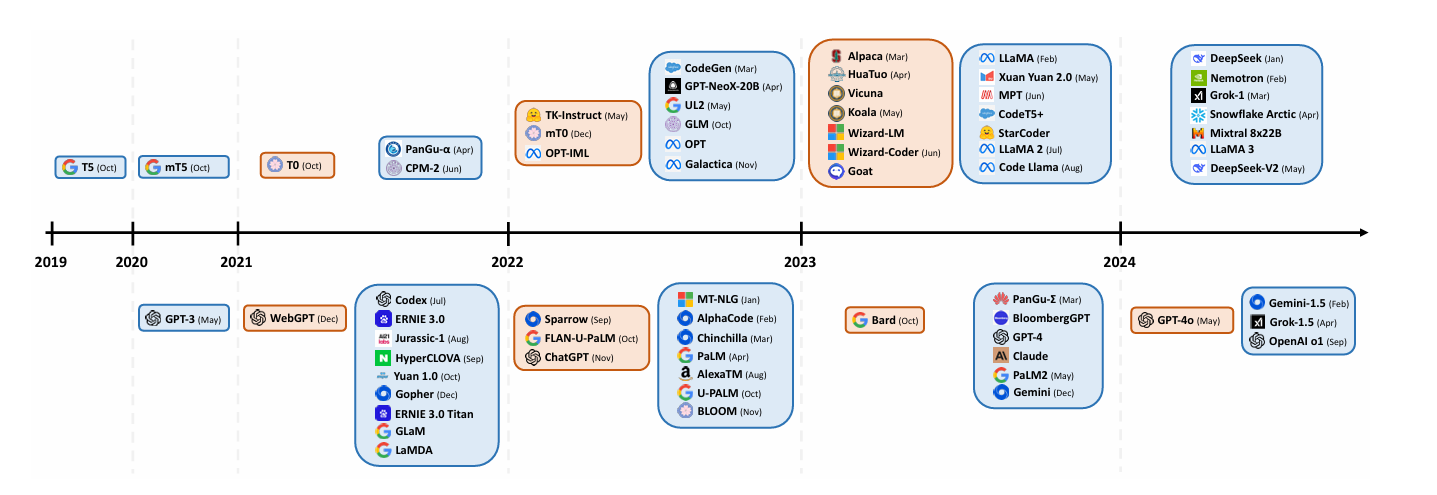
\includegraphics[width=0.85\textwidth, keepaspectratio]{Figures/llm_evolution.png}
    }{
        \framebox[0.85\textwidth]{\rule{0pt}{150pt} \textbf{Missing Image:} llm\_evolution.png}
    }
    \caption{The evolution of Large Language Models.}
    \label{fig:llm_evolution}
\end{figure}

\subsection{Advancements and Capabilities}
LLMs have demonstrated emergent abilities—such as zero-shot reasoning, logical decision-making, and in-context learning—which arise from their massive scale rather than explicit task-specific training. These capabilities allow LLMs to perform complex operations with minimal task-specific data, showcasing their profound generalization potential. Fine-tuning and alignment techniques (such as RLHF) further enhance their performance, enabling them to strictly follow user intent and generate highly accurate, safe responses. 

Moreover, LLMs have shown significant improvements in multi-tasking and adapting to novel contexts. This versatility has positioned them as indispensable tools across diverse industries, ranging from healthcare to finance and legal technology. These advancements underscore the growing importance of LLMs as the cognitive engines of modern AI-driven applications.

\subsection{Challenges and Opportunities}
Despite their undeniable success, LLMs face significant operational challenges, including high computational costs, slow inference latency, and substantial hardware requirements. These limitations have spurred intensive research into more efficient architectures, model compression techniques, and parameter-efficient fine-tuning strategies designed to make LLMs more accessible and practical for broader commercial applications. Methods such as model distillation, structured pruning, and weight quantization are actively being explored to reduce the immense resource intensity of these models. 

One of the most critical challenges LLMs face is managing large-scale input data. While state-of-the-art LLMs can possess context windows of up to 2 million tokens, enterprise knowledge bases often span millions of documents, dwarfing these limits. This discrepancy restricts the ability of LLMs to process entire organizational datasets directly in a single inference step, complicating tasks that require simultaneous access to vast, dispersed information. 

Additionally, the processing time for an LLM query is highly sensitive to the length of the input context. Longer queries demand significantly more computation because the self-attention mechanism processes each token, resulting in increased latency and higher financial costs. Consequently, handling extremely long contexts can become prohibitively expensive, particularly for applications requiring real-time responsiveness or frequent large-scale queries. 

Furthermore, ensuring the ethical deployment of LLMs, mitigating algorithmic biases, and preventing the generation of misleading or harmful outputs remain critical concerns. Overcoming these hurdles presents rich opportunities for ongoing research and engineering innovation.

\begin{table}[H]
    \centering
    \resizebox{\textwidth}{!}{
    \begin{tabular}{l c c c c}
        \toprule
        \textbf{Model} & \textbf{Context Window} & \textbf{Cost (USD/1M Tokens)} & \textbf{Tokens/s} & \textbf{First Chunk (s)} \\
        \midrule
        GPT-4o & 128k & \$7.50 & 97.4 & 0.45 \\
        GPT-4 Turbo & 128k & \$15.00 & 31.9 & 0.60 \\
        GPT-3.5 Turbo & 16k & \$0.75 & 88.6 & 0.38 \\
        Gemini 1.5 Pro & 2M & \$5.25 & 64.6 & 1.05 \\
        Llama 3.1 405B & 128k & \$4.50 & 29.4 & 0.66 \\
        Claude 3.5 Sonnet & 200k & \$6.00 & 76.5 & 1.32 \\
        Mistral Large 2 & 128k & \$4.50 & 36.8 & 0.51 \\
        Mixtral 8x22B & 65k & \$1.20 & 63.3 & 0.34 \\
        \bottomrule
    \end{tabular}
    }
    \caption{Comparison of Selected Models Based on Context Window, Cost, and Performance.}
    \label{tab:model_comparison}
\end{table}

\subsection{Conclusion}
LLMs represent a monumental advancement in Natural Language Processing, offering unprecedented capabilities in text comprehension and generation. However, the operational challenges associated with their deployment—including computational efficiency, context window limitations, query processing latency, and ethical considerations—highlight the pressing need for continued innovation in model architecture and augmentation methodologies.

\section{Vector Stores}

\subsection{Introduction}
While LLMs have made significant strides, their inherent limitations in handling vast amounts of raw input data and long-tail queries remain a crucial bottleneck. Fortunately, emerging architectural paradigms are addressing this issue by providing highly sophisticated mechanisms for managing and accessing large-scale information dynamically during inference. These advancements promise to unlock the full potential of LLMs, enabling them to bypass strict token limits. In the following sections, we will explore vector storage—a groundbreaking architecture that fundamentally redefines large-scale data retrieval for generative AI models.

\subsection{Embeddings and Their Importance}
A vector store is a specialized database engineered to store and efficiently query dense vector embeddings, which are high-dimensional mathematical representations of unstructured data. These embeddings accurately capture the semantic meaning of complex information—such as text, images, or audio—and are paramount for applications requiring rapid, context-aware information retrieval based on semantic similarity rather than mere keyword matching.

Embeddings distill the semantic and syntactic content of data into a continuous vector space that machine learning models can process optimally. They empower systems to execute semantic searches by calculating the mathematical distance (e.g., cosine similarity) between vectors in high-dimensional space. Typically generated by deep neural networks such as BERT or BGE, these vectors encode the intricate relationships between distinct concepts. 

Within this vector space, semantically similar concepts are positioned in close geometric proximity. For instance, synonyms like "contract" and "agreement" would yield embeddings located near one another, reflecting their shared contextual meaning. This capability is absolutely essential for applications demanding high-precision, contextually relevant information retrieval.

\begin{figure}[H]
    \centering
    \IfFileExists{Figures/embedding_space.png}{
        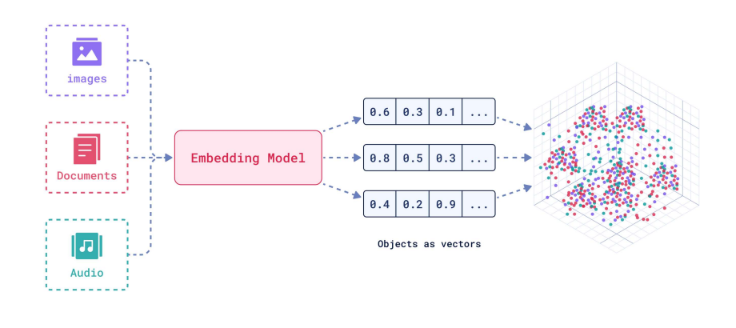
\includegraphics[width=0.7\textwidth, keepaspectratio]{Figures/embedding_space.png}
    }{
        \framebox[0.7\textwidth]{\rule{0pt}{150pt} \textbf{Missing Image:} embedding\_space.png}
    }
    \caption{Illustration of embedding vectors in a high-dimensional semantic space.}
    \label{fig:embedding_space}
\end{figure}

\subsection{Memory and Efficiency Considerations}
The high-dimensional nature of vector embeddings—often consisting of hundreds or thousands of floating-point dimensions—can impose severe memory constraints on the hosting infrastructure. For example, a single 1024-dimensional vector stored as 32-bit floating-point numbers requires approximately 4 KB of memory. As an enterprise database scales into millions of vectors, the active memory demands become substantial. 

To mitigate these memory overheads and accelerate retrieval speeds, sophisticated techniques such as Product Quantization or Binary Quantization are frequently employed. These approaches compress the vectors, drastically reducing their memory footprint while preserving sufficient topological information to guarantee effective retrieval. Converting a 1536-dimensional vector to a binary format, for instance, can reduce its memory requirement by a factor of 40, concurrently accelerating the dot-product calculations required for search. Despite this aggressive compression, high recall accuracy can be maintained by implementing a two-stage pipeline: utilizing compressed vectors for the initial rapid search, and full-precision vectors (or Cross-Encoders) for final ranking.

\subsection{HNSW Algorithm in Vector Stores}
The Hierarchical Navigable Small World (HNSW) algorithm is a state-of-the-art methodology for Approximate Nearest Neighbor (ANN) search, significantly augmenting the query performance of modern vector stores. Traditional brute-force search approaches possess a time complexity of $\mathcal{O}(N)$, rendering them highly impractical for massive datasets. HNSW successfully reduces this search complexity to $\mathcal{O}(\log N)$, enabling sub-millisecond retrieval times. 

The HNSW algorithm organizes vector data into multiple hierarchical layers, each representing a varying level of abstraction and connectivity. The foundational bottom layer contains all data points and is densely interconnected, whereas the upper layers contain exponentially fewer points and longer connections, forming a navigational hierarchy. During a search, the algorithm traverses the sparse upper layers to rapidly locate the general vicinity of the target. Once this approximate region is identified, the search cascades into the denser lower layers to pinpoint the exact nearest neighbors.

The spatial memory complexity of HNSW remains $\mathcal{O}(N)$, as each embedded point maintains a fixed maximum number of connections, ensuring memory consumption grows linearly rather than exponentially. This architectural elegance makes HNSW the industry standard for large-scale, high-velocity semantic retrieval.

\begin{figure}[H]
    \centering
    \IfFileExists{Figures/hnsw_layers.png}{
        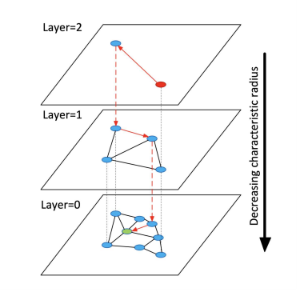
\includegraphics[width=0.75\textwidth, keepaspectratio]{Figures/hnsw_layers.png}
    }{
        \framebox[0.75\textwidth]{\rule{0pt}{150pt} \textbf{Missing Image:} hnsw\_layers.png}
    }
    \caption{Hierarchical representation of the HNSW algorithm layers used in modern Vector Databases.}
    \label{fig:hnsw_layers}
\end{figure}

\subsection{Conclusion}
Vector stores, powered by indexing algorithms like HNSW, represent a paradigm shift in data retrieval technology. By leveraging dense high-dimensional embeddings and logarithmic search algorithms, vector databases offer unparalleled performance for tasks requiring deep semantic understanding. While they demand more active memory than traditional relational databases, vector stores provide the critical speed and accuracy necessary to support next-generation AI applications, from enterprise semantic search to robust data analysis.

\section{RAG Architecture}

\subsection{Introduction}
Large pre-trained language models excel at internalizing vast quantities of factual knowledge within their parameters, achieving remarkable zero-shot performance across various NLP domains. However, they frequently struggle to access and manipulate this latent knowledge accurately, particularly in knowledge-intensive or highly specialized tasks (such as legal reasoning). This architectural limitation becomes glaringly evident when models hallucinate facts, fail to provide up-to-date information, lack the ability to cite provenance for their outputs, or require constant, expensive retraining to update their internal knowledge base. 

Retrieval-Augmented Generation (RAG) elegantly resolves these fundamental challenges by integrating pre-trained parametric memory (the LLM) with dynamic, non-parametric memory (a vector database). In a RAG architecture, a generative model is actively fed by a neural retriever that searches a dense vector index representing a massive external corpus (e.g., millions of legal documents). This architecture empowers the system to dynamically fetch the most relevant, up-to-date information strictly during the inference generation process, resulting in highly specific, diverse, and empirically factual outputs. 

By injecting a deterministic retrieval mechanism directly into the prompt pipeline, RAG models consistently demonstrate state-of-the-art performance in complex NLP tasks, dramatically outperforming parametric-only models while completely resolving the issues of knowledge provenance and hallucination.

\begin{figure}[H]
    \centering
    \IfFileExists{Figures/rag_architecture.jpg}{
        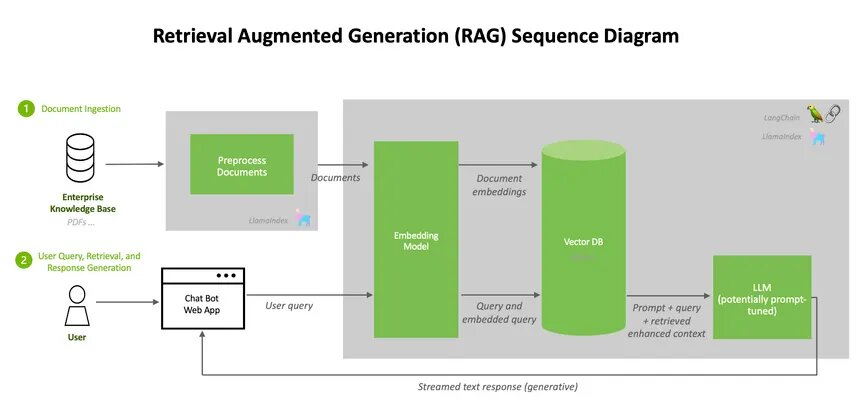
\includegraphics[width=0.85\textwidth, keepaspectratio]{Figures/rag_architecture.jpg}
    }{
        \framebox[0.85\textwidth]{\rule{0pt}{150pt} \textbf{Missing Image:} rag\_architecture.jpg}
    }
    \caption{The standard Retrieval-Augmented Generation (RAG) architecture combining an LLM with an external vector retrieval mechanism.}
    \label{fig:rag_architecture}
\end{figure}

\subsection{The Necessity of RAG Architecture}
Traditional language models rely exclusively on the static information encoded within their neural weights during the pre-training phase. While these models perform admirably on general conversational tasks, they fail critically on tasks demanding domain-specific, proprietary, or temporally recent information. An un-augmented model will frequently generate outdated or entirely fabricated responses because the knowledge it acquired during pre-training is inherently frozen in time and inherently generalized. 

RAG architectures mitigate these limitations by decoupling knowledge storage from language generation. By integrating a dedicated retrieval mechanism, the model is permitted to query external, proprietary knowledge bases on-the-fly. This guarantees that the LLM is constantly grounded by accurate, contextually appropriate, and highly pertinent data fetched directly from a verified repository, effectively turning the LLM from a "memorizer" into an advanced "synthesizer" of factual information.

\subsection{Conclusion}
The RAG architecture, fundamentally underpinned by high-performance vector stores, constitutes a major breakthrough in the deployment of Enterprise AI. By fusing the reasoning capabilities of pre-trained language models with the deterministic accuracy of semantic retrieval mechanisms, RAG guarantees the generation of contextually aware and factually grounded outputs. Consequently, RAG serves as the definitive architecture for deploying secure, trustworthy AI applications in critical sectors such as law, medicine, and finance.

\chapter{Project Context and Objectives}
\label{chap:Project_Context_and_Objectives}

\section*{Introduction}
This chapter delineates the foundational context of the project, elucidates the specific challenges it seeks to address, and establishes the primary objectives that will guide the development of the proposed LegalTech platform.

\section{General Project Framework}

\subsection{General Context}
The contemporary global landscape is characterized by a rapid acceleration in digital transformation, presenting unprecedented opportunities to automate and optimize diverse sectors. However, the legal and administrative domain—particularly within Morocco—remains heavily reliant on traditional, manual methodologies. This pervasive reliance on legacy systems renders the acquisition of accurate legal information and the execution of administrative consultations inherently complex, financially burdensome, and highly resource-intensive.

As first-year engineering students enrolled in the "Advanced Software Engineering for Digital Services" (ASEDS) program at the National Institute of Posts and Telecommunications (INPT), we have cultivated a robust academic foundation encompassing software engineering principles, advanced database management, and the architecture of complex digital systems \cite{ref2}. Capitalizing on this foundation and the ongoing revolution in artificial intelligence, we identified a compelling opportunity to harness these emerging technologies. By focusing specifically on the LegalTech domain, we aim to modernize this critical sector, facilitating seamless, reliable, and democratized access to legal information for the general public.

\subsection{Problem Statement}
Despite the pressing need to digitize the legal sector, the integration of artificial intelligence into the Moroccan legal framework encounters several distinct technical and economic hurdles. These challenges can be synthesized as follows:

\begin{itemize}
    \item \textbf{Prohibitive Costs and Automation Deficits:} The systemic lack of automation in the legal sector renders professional consultations prohibitively expensive. Legal consultants typically mandate substantial fees, presenting the average user with a severe dilemma: either expend inordinate hours conducting manual, often fruitless web searches, or incur exorbitant costs for a fundamental legal inquiry.
    
    \item \textbf{Limitations of Global LLMs (The Hallucination Risk):} Despite the extraordinary capabilities of Large Language Models (LLMs), these architectures are predominantly trained on foreign, anglo-centric datasets and inherently lack deep, localized knowledge of Moroccan legal jurisprudence. Consequently, when queried regarding specific Moroccan legal procedures, these models frequently succumb to "hallucinations," generating confident but entirely fabricated and factually incorrect responses.
    
    \item \textbf{Data Extraction Bottlenecks (Unstructured Document Formats):} Moroccan legal documents and administrative circulars are rarely distributed in machine-readable, digital-native formats. Instead, they predominantly exist as scanned, image-based PDF files replete with complex tabular matrices, official stamps, and handwritten signatures. Traditional Optical Character Recognition (OCR) heuristics consistently fail to process and accurately extract structured semantic data from these artifacts.
    
    \item \textbf{Linguistic and Semantic Barriers:} The vast majority of official documentation is drafted in formal, highly structured Legal Arabic. Processing this specific dialect necessitates a robust, specialized Embedding Model explicitly trained on Arabic semantic structures to execute accurate mathematical vector searches.
\end{itemize}

\subsection{Project Objectives}
In direct response to these multi-faceted challenges, this project endeavors to architect and deploy an integrated digital platform. The successful realization of this platform is predicated on achieving the following primary and secondary objectives:

\begin{itemize}
    \item Conduct a rigorous needs analysis and formally draft a comprehensive project specifications document.
    \item Evaluate and select an optimal, modern technology stack capable of supporting high-performance enterprise requirements.
    \item Architect an advanced Retrieval-Augmented Generation (RAG) system specifically designed to eradicate AI hallucination by forcing the generative model to synthesize answers exclusively from verified Moroccan legal sources.
    \item Implement state-of-the-art OCR pipelines and multilingual Embedding Models to ensure high-fidelity data ingestion.
    \item Develop an intuitive, responsive User Interface (UI) featuring:
    \begin{itemize}
        \item A real-time chat interface allowing users to converse dynamically with the RAG-powered Legal LLM.
        \item A multimodal bypass system empowering users to upload and query their personal documents directly.
        \item A Split-Screen \LaTeX\ Editor enabling users to autonomously draft, modify, and compile professional legal documents via code or through AI-driven template injection.
    \end{itemize}
    \item Implement a robust Identity and Access Management (IAM) system for secure authentication.
    \item Enforce strict data security and Row-Level Security (RLS) policies to protect user metadata and uploaded artifacts.
    \item Design a highly normalized, asynchronous relational database.
    \item Engineer a comprehensive, JSON-based telemetry and logging system to monitor backend execution and AI latencies.
    \item Optimize backend concurrency to support high-volume parallel requests while minimizing operational cloud costs.
    \item Execute exhaustive Quality Assurance (QA) and end-to-end testing protocols to guarantee systemic stability.
    \item Finalize and execute the production deployment of the platform.
\end{itemize}

\newpage
\section{Project Management and Methodology}

\subsection{Adopted Methodology}

\subsubsection{The Scrum Framework}
Scrum is an agile organizational framework utilized to manage the development of complex products. Defined by its creators as an iterative, holistic framework, Scrum focuses on achieving common objectives by delivering high-value products in a productive and creative manner. It is widely recognized as a premier implementation of the Agile Manifesto's core principles.

\begin{figure}[htbp]
    \centering
    \IfFileExists{Figures/1.jpg}{
        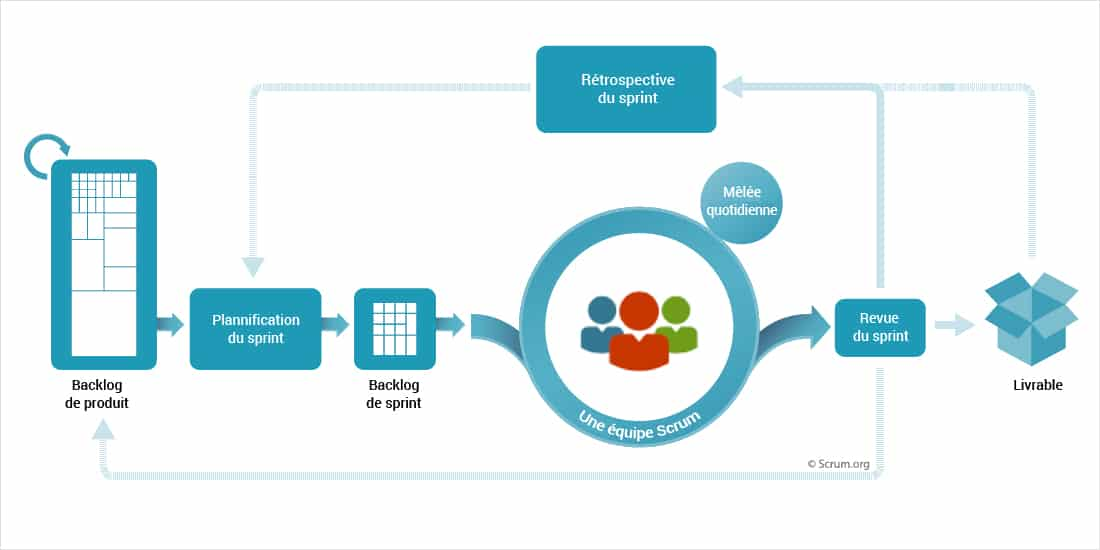
\includegraphics[width=0.85\textwidth, keepaspectratio]{Figures/1.jpg}
    }{
        \framebox[0.85\textwidth]{\rule{0pt}{150pt} \textbf{Missing Image: Figures/1.jpg}}
    }
    \caption{Visual representation of the Scrum Agile methodology.}
    \label{fig:scrum_schema}
\end{figure}

Implementing a project under Scrum best practices requires the following foundational elements:
\begin{itemize}
    \item An autonomous, highly responsible cross-functional team capable of rapidly adapting to dynamic client requirements or pivoting technical scopes.
    \item A structural workflow organized into "Sprints": short, time-boxed iterations (typically 2 to 4 weeks) facilitating rapid intervention and continuous integration.
    \item A rigorous definition of requirements, systematically consolidated into an evolving master task list known as the "Product Backlog."
\end{itemize}

\subsubsection{Roles within Scrum}
The Scrum framework prescribes three primary roles:
\begin{enumerate}[label=\arabic*)]
    \item \textbf{The Product Owner:} The product's visionary and the primary proxy for the client's expectations. This role mandates high availability to resolve ambiguities and prioritize the backlog.
    \item \textbf{The Scrum Master:} The facilitator responsible for ensuring absolute adherence to Scrum values. The Scrum Master shields the team from external disruptions and orchestrates the removal of developmental bottlenecks.
    \item \textbf{The Development Team:} A self-managing, autonomous collective devoid of internal hierarchical structures, where technical decisions are deliberated and executed collaboratively.
\end{enumerate}

These entities synergize to execute the following core Scrum events:
\begin{itemize}
    \item \textbf{The Sprint:} A strict time-box defining the developmental cycle.
    \item \textbf{Sprint Planning:} The initial event where the team collaboratively selects specific User Stories from the Product Backlog to target during the impending Sprint.
    \item \textbf{Sprint Execution:} The active developmental phase, encompassing architectural design, programming, and testing.
    \item \textbf{Sprint Review and Retrospective:} The concluding evaluation where the team demonstrates the newly implemented features and introspects on workflow improvements for subsequent Sprints.
    \item \textbf{Backlog Grooming:} The continuous refinement and re-prioritization of the Product Backlog to accommodate shifting project dynamics.
\end{itemize}

\subsection{Role Distribution within the Team}
Given the streamlined nature of our academic development team for this project, the allocation of a dedicated, full-time Scrum Master was structurally impractical. Consequently, we adopted an adapted, highly collaborative Scrum paradigm, dynamically distributing the responsibilities of the Product Owner, Scrum Master, and Developers amongst ourselves to best simulate enterprise Agile workflows.

\subsection{Collaboration and Communication Tools}

\subsubsection{Instant Communication}
We utilized direct messaging platforms (such as WhatsApp) as our primary conduit for rapid coordination, conducting four distinct types of Agile meetings:
\begin{itemize}
    \item \textbf{Daily Stand-ups:} Brief syncs allowing team members to report progress, highlight immediate goals, and flag technical blockers.
    \item \textbf{Pair-Programming Syncs:} Technical deep-dives utilized for complex architectural design and collaborative debugging sessions.
    \item \textbf{Product Demonstration Reviews:} Milestone meetings dedicated to showcasing compiled features and reviewing the project's holistic functionality prior to final delivery.
\end{itemize}

\begin{figure}[htbp]
    \centering
    \IfFileExists{Figures/2.png}{
        
\includegraphics[width=0.4\textwidth, keepaspectratio]{Figures/2.png}
    }{
        \framebox[0.4\textwidth]{\rule{0pt}{100pt} \textbf{Missing Image: Figures/2.png}}
    }
    \caption{Example of team communication and daily stand-ups.}
    \label{fig:communication}
\end{figure}

\subsubsection{Version Control and Source Management}
We strictly enforced version control methodologies utilizing \textbf{Git} and \textbf{GitHub}. This centralized approach guaranteed that the entire team maintained synchronized access to the latest verified codebase. 

We adopted a strict \textbf{Branching and Merging} strategy, ensuring features were isolated during development and only merged into the main production branch following rigorous peer review. Furthermore, every \textbf{Commit} was carefully documented with descriptive syntax, ensuring absolute traceability of the platform's evolutionary history, as illustrated below.

\begin{figure}[htbp]
    \centering
    \IfFileExists{Figures/3.png}{
        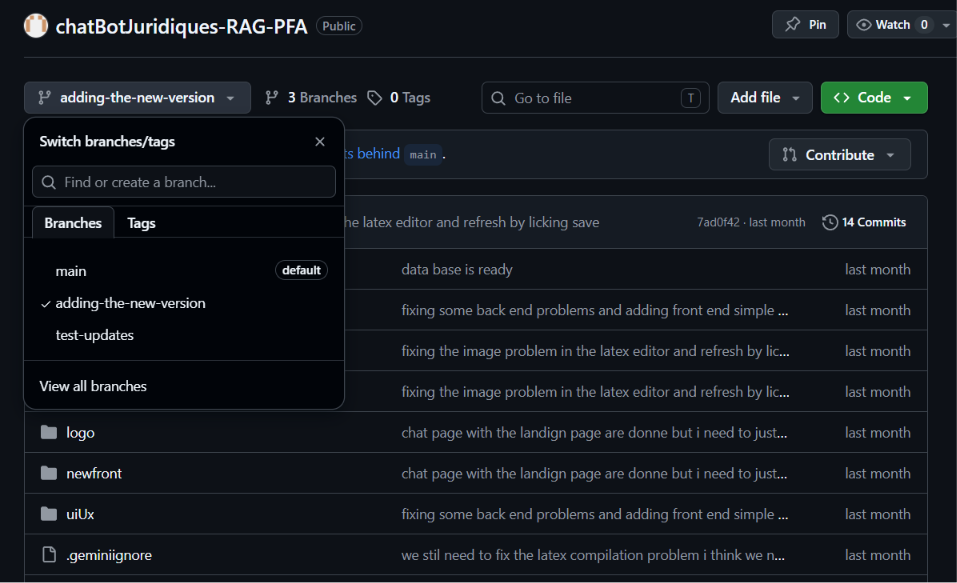
\includegraphics[width=0.9\textwidth, keepaspectratio]{Figures/3.png}
    }{
        \framebox[0.9\textwidth]{\rule{0pt}{150pt} \textbf{Missing Image: Figures/3.png}}
    }
    \caption{Version control trace highlighting Git commits and branches on GitHub.}
    \label{fig:github_commits}
\end{figure}

\section*{Conclusion}
Having firmly established the systemic context, diagnosed the core industry bottlenecks, and articulated the definitive objectives required for project success, the theoretical framework of the LegalTech platform is complete. The subsequent chapters will detail the precise needs specification, the system modeling, and the highly optimized architectural design required to materialize this vision.

\chapter{Analysis and Specifications}
\label{chap:Analysis_and_Specifications}

\section*{Introduction}
This chapter is dedicated to delineating the detailed specifications and requirements of the proposed LegalTech platform. A rigorous analysis is essential to ensure the system architecture aligns with both the overarching project objectives and the specific expectations of end-users. In the subsequent sections, we categorize these specifications into functional requirements, detailing the explicit capabilities the system must exhibit; non-functional requirements, outlining the performance and operational standards; and system constraints, which establish the developmental, financial, and technological boundaries.

\newpage

\section{Functional Requirements}
This section enumerates the functional requirements foundational to the platform's architecture. These represent the core features and behaviors the system must support to facilitate a robust, AI-powered legal application.

\subsection{User Interface (UI)}
\begin{itemize}
    \item \textbf{Landing Page:} The platform shall provide an intuitive, user-centric landing page that clearly articulates the application's core concept, value proposition, and primary functionalities.
    \item \textbf{Account Creation \& Login:} Users must be empowered to create an account and authenticate securely utilizing multiple Identity Providers (IdPs), including Email/Password, Google, Facebook, and Apple ID.
    \item \textbf{AI Chat Interface:} A dedicated conversational interface must be provisioned, allowing users to interact directly with the Large Language Model (LLM) augmented by the RAG pipeline.
    \item \textbf{File Upload \& Management:} Users must be able to upload personal documents directly into the chat interface. Additionally, they require a persistent, personal cloud repository to store documents and import them into active chat sessions on demand.
    \item \textbf{Document Generation:} The platform shall enable users to draft formal legal documents manually using \LaTeX\ via direct code input within an integrated IDE.
    \item \textbf{AI-Assisted Drafting:} Users shall have the ability to prompt the AI assistant to autonomously draft, format, or modify legal documents utilizing a centralized registry of pre-existing templates.
\end{itemize}

\subsection{Large Language Model (LLM) Integration}
\begin{itemize}
    \item \textbf{Model Selection:} The platform must seamlessly integrate a highly capable, state-of-the-art LLM optimized for complex legal reasoning and multilingual comprehension.
    \item \textbf{Context Memory:} The conversational agent must retain conversational context, effectively remembering previous prompts and uploaded documents within a contiguous session.
    \item \textbf{Role Prompting:} The LLM must be strictly governed by engineered system prompts, enforcing rigorous rules and constraints to ensure it consistently operates within its designated persona as a Moroccan legal assistant.
\end{itemize}

\subsection{Data Retrieval (RAG System)}
\begin{itemize}
    \item \textbf{RAG Architecture:} A Retrieval-Augmented Generation (RAG) paradigm shall be implemented to synthesize LLM-generated responses with highly relevant, empirically factual data extracted from a curated document corpus.
    \item \textbf{Standardized Retrieval Mechanism:} The system shall leverage specialized Vector Stores (ChromaDB) to facilitate rapid, efficient, and semantically precise searches based on user queries.
\end{itemize}

\subsection{Authentication and Authorization}
\begin{itemize}
    \item \textbf{Multi-Provider Auth:} The system must implement robust, enterprise-grade authentication by integrating third-party OAuth providers via Clerk.
    \item \textbf{Admin Dashboard:} A secure, restricted-access dashboard must be exclusively available to platform administrators for user governance and systemic monitoring.
\end{itemize}

\subsection{System Monitoring and Reporting}
\begin{itemize}
    \item \textbf{Smart Logging System:} An automated, highly structured telemetry mechanism must be implemented. To optimize disk storage, logs shall be compressed into \texttt{.gz} archives daily and subjected to a 30-day rolling deletion policy.
    \item \textbf{Automated API Retry Mechanism:} To minimize error rates and ensure high availability, backend controllers must autonomously retry transiently failed API requests prior to propagating errors to the client.
\end{itemize}

\section{Non-Functional Requirements}
This section outlines the non-functional requirements that dictate the operational behavior of the architecture, focusing heavily on critical attributes such as performance, scalability, and security.

\subsection{Performance}
\begin{itemize}
    \item \textbf{Concurrency:} The application infrastructure must efficiently handle up to 100 concurrent user sessions without experiencing degradation in service quality.
    \item \textbf{Response Time:} The RAG pipeline and LLM inference engine must deliver responses to complex queries within a maximum threshold of 120 seconds.
    \item \textbf{Input Handling:} The architecture must be optimized to process massive input payloads (e.g., multimodal prompts or raw document text exceeding 10,000 characters) without catastrophic performance bottlenecks.
\end{itemize}

\subsection{Scalability}
\begin{itemize}
    \item \textbf{Horizontal Scaling:} The architecture shall be intrinsically scalable, permitting the platform to dynamically augment capacity by spinning up additional instances of core components (e.g., FastAPI workers, vector databases).
\end{itemize}

\subsection{Security}
\begin{itemize}
    \item \textbf{Data Protection:} The platform must enforce industry-standard encryption protocols (TLS/SSL) for data in transit and secure persistence mechanisms for data at rest.
    \item \textbf{Vulnerability Mitigation:} The application infrastructure must be rigorously protected against pervasive web vulnerabilities, specifically Distributed Denial of Service (DDoS) attacks and SQL Injection.
\end{itemize}

\section{System Constraints}
Constraints delineate the mandatory boundaries and operational limitations within which the project must be engineered and maintained.

\subsection{Budget Constraints}
\begin{itemize}
    \item \textbf{Cost Optimization:} The architecture must be meticulously optimized for financial efficiency, minimizing long-term operational expenditures related to API token usage and cloud hosting.
    \item \textbf{Flexible Deployment:} The architecture must be containerized or highly portable to support flexible deployment options, facilitating rapid migration to cost-effective hosting providers if economically necessary.
\end{itemize}

\subsection{Time Constraints}
\begin{itemize}
    \item \textbf{Development Timeline:} While the underlying architecture is designed for long-term extensibility, the complete development, testing, and deployment cycle of this iteration must strictly adhere to a 3-month academic project timeline.
\end{itemize}

\subsection{Technological Constraints}
\begin{itemize}
    \item \textbf{Pre-Approved Tech Stack:} The system architecture must strictly conform to a pre-approved technology stack: \textbf{Python} (FastAPI) for all backend services and AI orchestration, and \textbf{React} (Vite) for all frontend client development.
    \item \textbf{Stack Deviations:} Any deviation from or addendum to the core technology stack must be rigorously justified and formally approved by project stakeholders.
\end{itemize}

\section{System Modeling (UML)}
\subsection{Use Case Actors}
An actor specifies a role played by a user or any external system that interacts directly with the subject. Actors are always external to the system boundaries, initiating use cases, providing inputs, or receiving outputs.

Within our platform ecosystem, the following actors have been identified:

\subsubsection*{Human Actors}
\begin{itemize}
    \item \textbf{User:} The primary end-user of the platform. This actor manages their profile, interacts with the AI chatbot, uploads legal documents, and compiles \LaTeX\ templates into final PDF artifacts.
    \item \textbf{Administrator:} A privileged user entrusted with the overarching governance of the platform. They possess the authority to oversee, control, and audit registered users and their respective access rights.
    \item \textbf{Log Responsible:} A specialized technical role dedicated to system maintenance. They are responsible for monitoring system telemetry, tracking runtime errors, and managing data retention policies to guarantee platform stability.
\end{itemize}

\subsubsection*{External Systems (External Actors)}
\begin{itemize}
    \item \textbf{Clerk Auth:} An external Identity and Access Management (IAM) provider invoked by the platform to securely broker user registration, authentication, and session generation.
    \item \textbf{Gemini LLM:} The external Large Language Model API that functions as the cognitive engine of the platform, executing context-aware legal reasoning and text generation.
    \item \textbf{GPT-4o OCR:} An external, AI-driven Vision model integrated specifically to perform high-fidelity Optical Character Recognition (OCR), extracting semantic text and Markdown tables from complex scanned documents.
    \item \textbf{LaTeXLite:} An external compilation engine service utilized by the workspace to seamlessly transpile user-generated \LaTeX\ code into rendered PDF documents.
\end{itemize}

\subsection{Use Case Diagram}
\begin{figure}[htbp]
    \centering
    \IfFileExists{Figures/use_case.png}{
        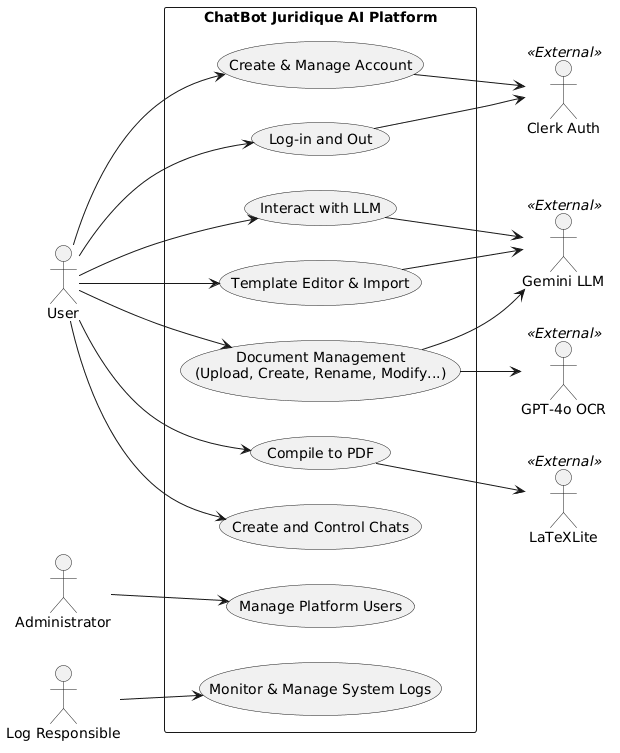
\includegraphics[width=0.75\textwidth, keepaspectratio]{Figures/use_case.png}
    }{
        \framebox[10cm]{\rule{0pt}{8cm} \textbf{Missing Image: Figures/use\_case.png}}
    }
    \caption{Global Use Case Diagram of the ChatBot Juridique AI Platform.}
    \label{fig:use_case_diagram}
\end{figure}

\newpage

\section{System Behavior (Sequence Diagrams)}
Sequence diagrams are imperative for visualizing the dynamic, temporal behavior of the system architecture. They meticulously map how internal components, backend APIs, and external services interact sequentially to execute the core functionalities of the platform.

\subsection{Chat Management and Live File Upload}
This sequence diagram comprehensively details the lifecycle of a chat session. It illustrates the workflow when a user initializes a new session, optionally uploads a live file (triggering a multimodal prompt bypass), transmits prompts to the RAG pipeline, and modifies chat metadata (e.g., renaming or pinning) via the FastAPI backend and PostgreSQL database.

\begin{figure}[H]
    \centering
    \IfFileExists{Figures/seq_chat_management.png}{
        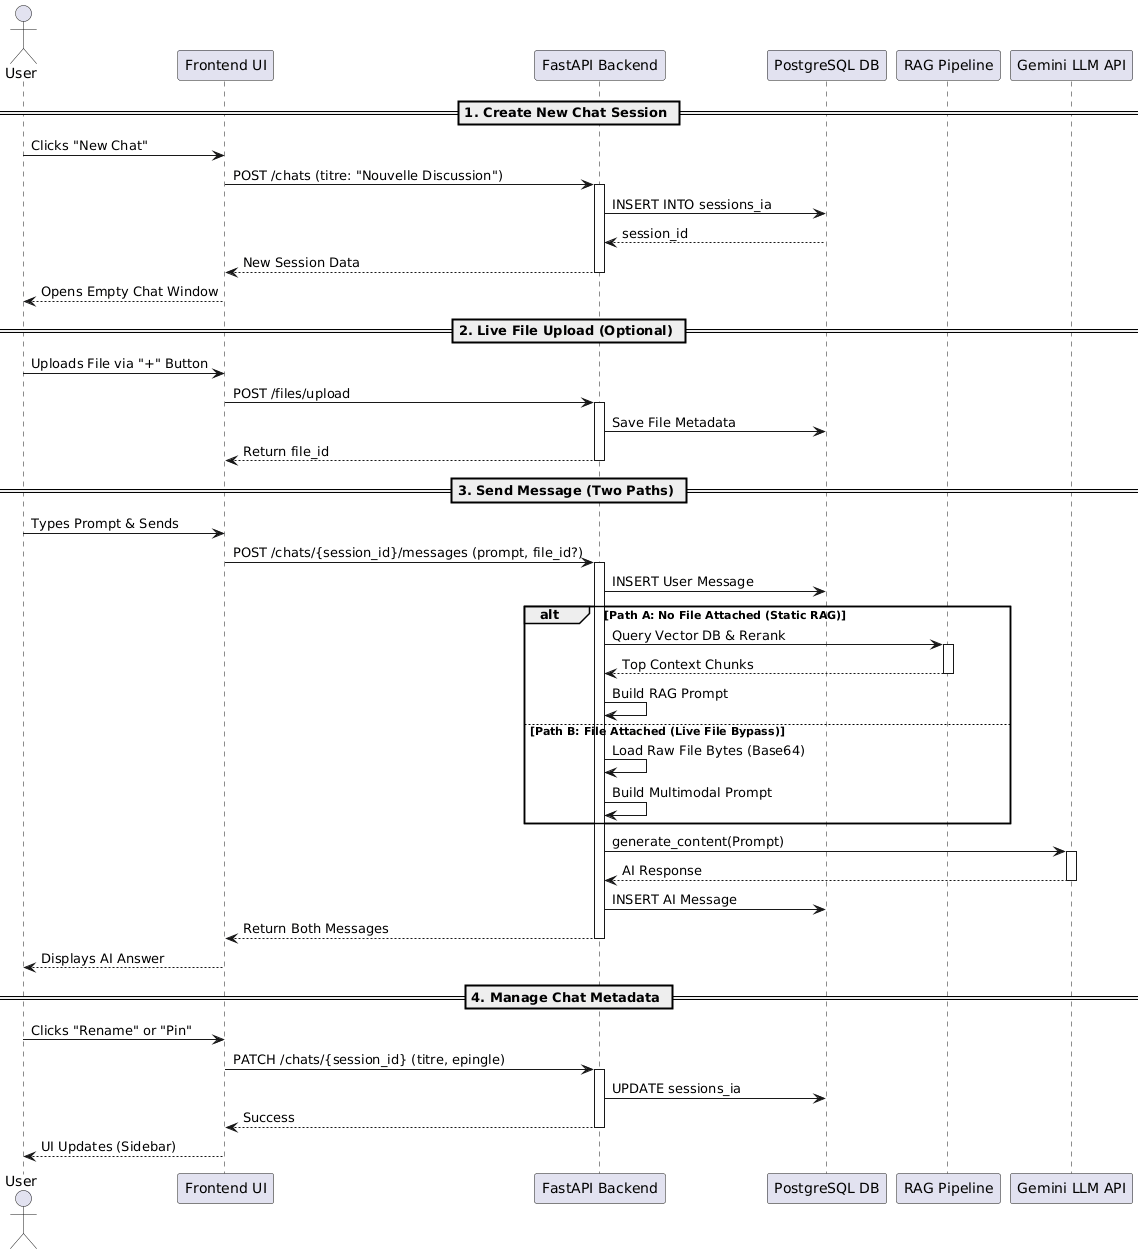
\includegraphics[width=0.9\textwidth, keepaspectratio]{Figures/seq_chat_management.png}
    }{
        \framebox[14cm]{\rule{0pt}{7cm} \textbf{Missing Image: Figures/seq\_chat\_management.png}}
    }
    \caption{Sequence Diagram illustrating Chat Session Management and Multimodal Interaction.}
    \label{fig:seq_chat_management}
\end{figure}

\newpage

\subsection{Core RAG Pipeline Execution}
This diagram maps the sophisticated query execution process when a user poses a legal question. It tracks the trajectory of the user's prompt as it is mathematically embedded, retrieved via cosine similarity in ChromaDB, rigorously reranked for maximum contextual relevance, and ultimately transmitted to the Gemini LLM to generate a factually grounded response.

\begin{figure}[H]
    \centering
    \IfFileExists{Figures/seq_rag_pipeline.png}{
        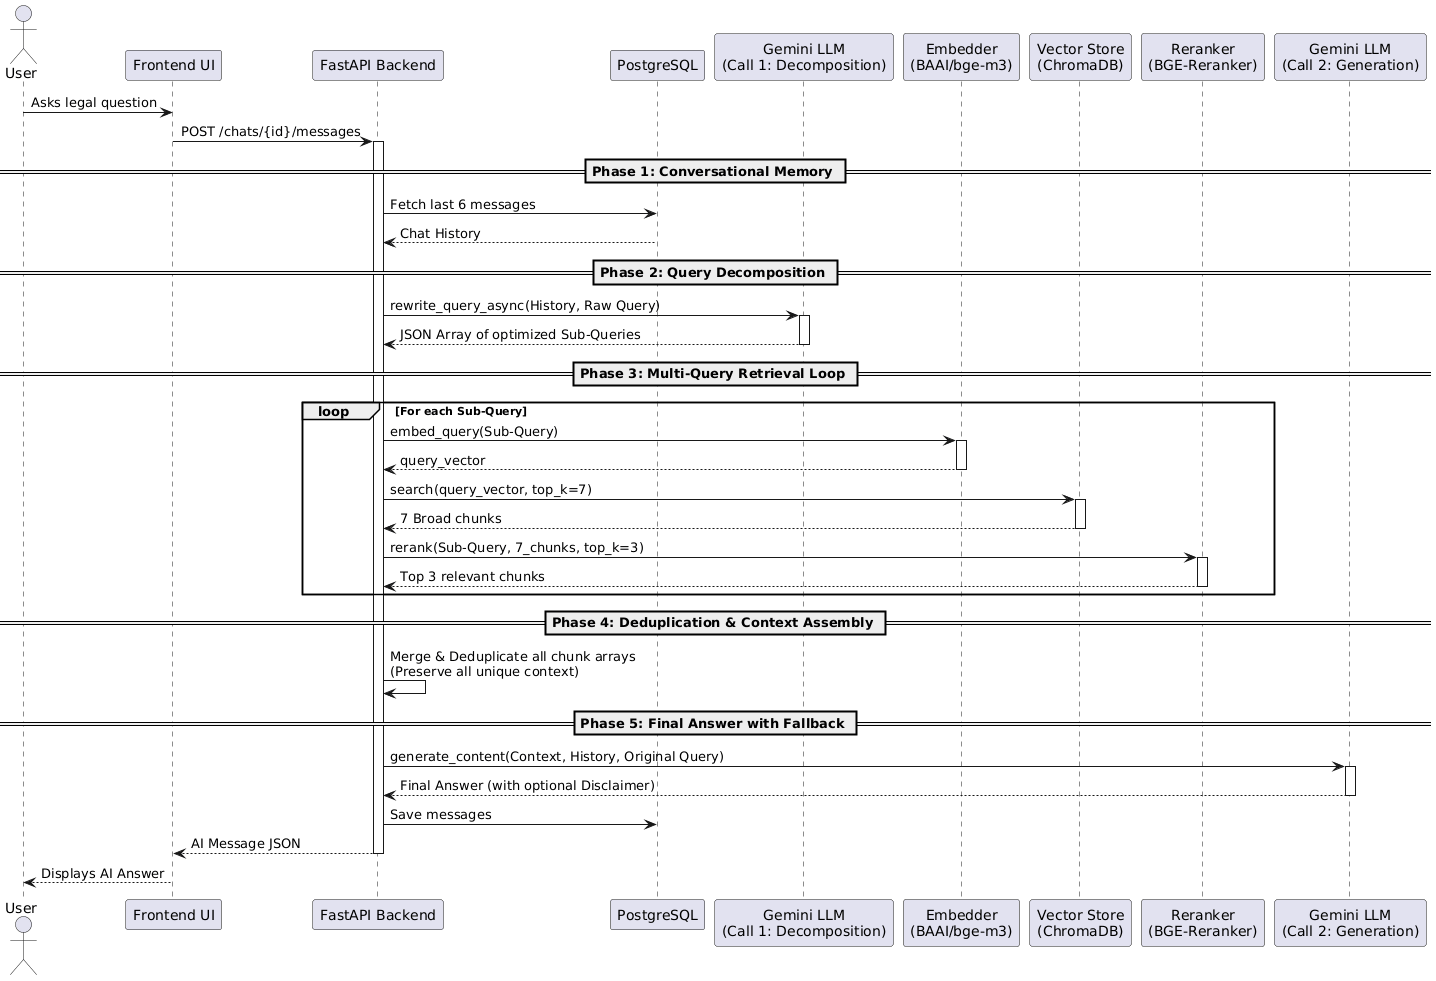
\includegraphics[width=0.9\textwidth, keepaspectratio]{Figures/seq_rag_pipeline.png}
    }{
        \framebox[14cm]{\rule{0pt}{7cm} \textbf{Missing Image: Figures/seq\_rag\_pipeline.png}}
    }
    \caption{Sequence Diagram of the Retrieval-Augmented Generation (RAG) Pipeline execution.}
    \label{fig:seq_rag}
\end{figure}

\newpage

\subsection{Document Upload and Data Ingestion}
This workflow details the highly complex offline data ingestion pipeline designed for Moroccan legal documents. It maps how raw PDFs are localized, converted into base64 images, processed by the GPT-4o Vision OCR to strip visual noise and extract semantic data, parsed by a custom XML chunker, and finally indexed into the vector database.

\begin{figure}[H]
    \centering
    \IfFileExists{Figures/seq_doc_upload.png}{
        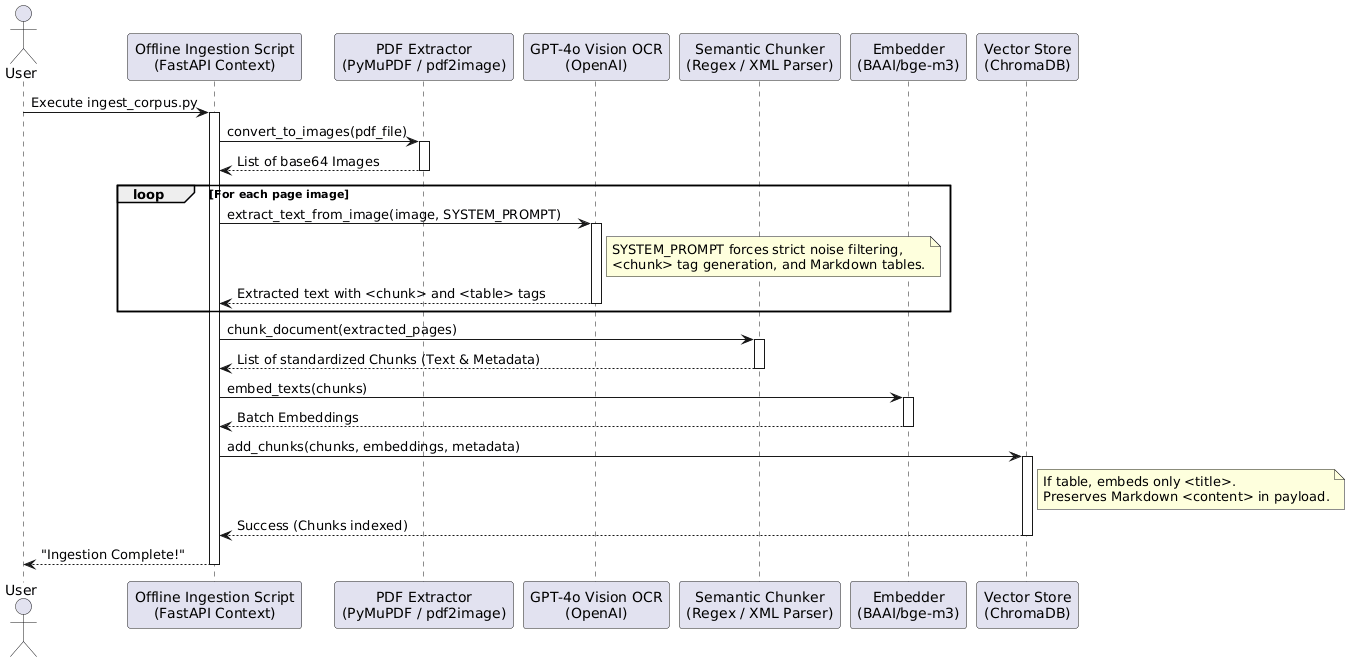
\includegraphics[width=0.9\textwidth, keepaspectratio]{Figures/seq_doc_upload.png}
    }{
        \framebox[14cm]{\rule{0pt}{7cm} \textbf{Missing Image: Figures/seq\_doc\_upload.png}}
    }
    \caption{Sequence Diagram of the Document Upload and AI-driven OCR Ingestion Process.}
    \label{fig:seq_upload}
\end{figure}

\vspace{1cm}

\subsection{AI-Assisted Document Generation}
This sequence diagram illustrates the \LaTeX\ document drafting and compilation feature. It maps how slash-commands (e.g., \texttt{/template}) trigger JSON template retrieval, which the LLM then adapts into syntactically valid \LaTeX\ code. Subsequently, it traces the dual-path compilation request—dynamically selecting between a local pdfLaTeX engine and the LaTeXLite cloud API—to render the final PDF.

\begin{figure}[H]
    \centering
    \IfFileExists{Figures/seq_doc_generation.png}{
        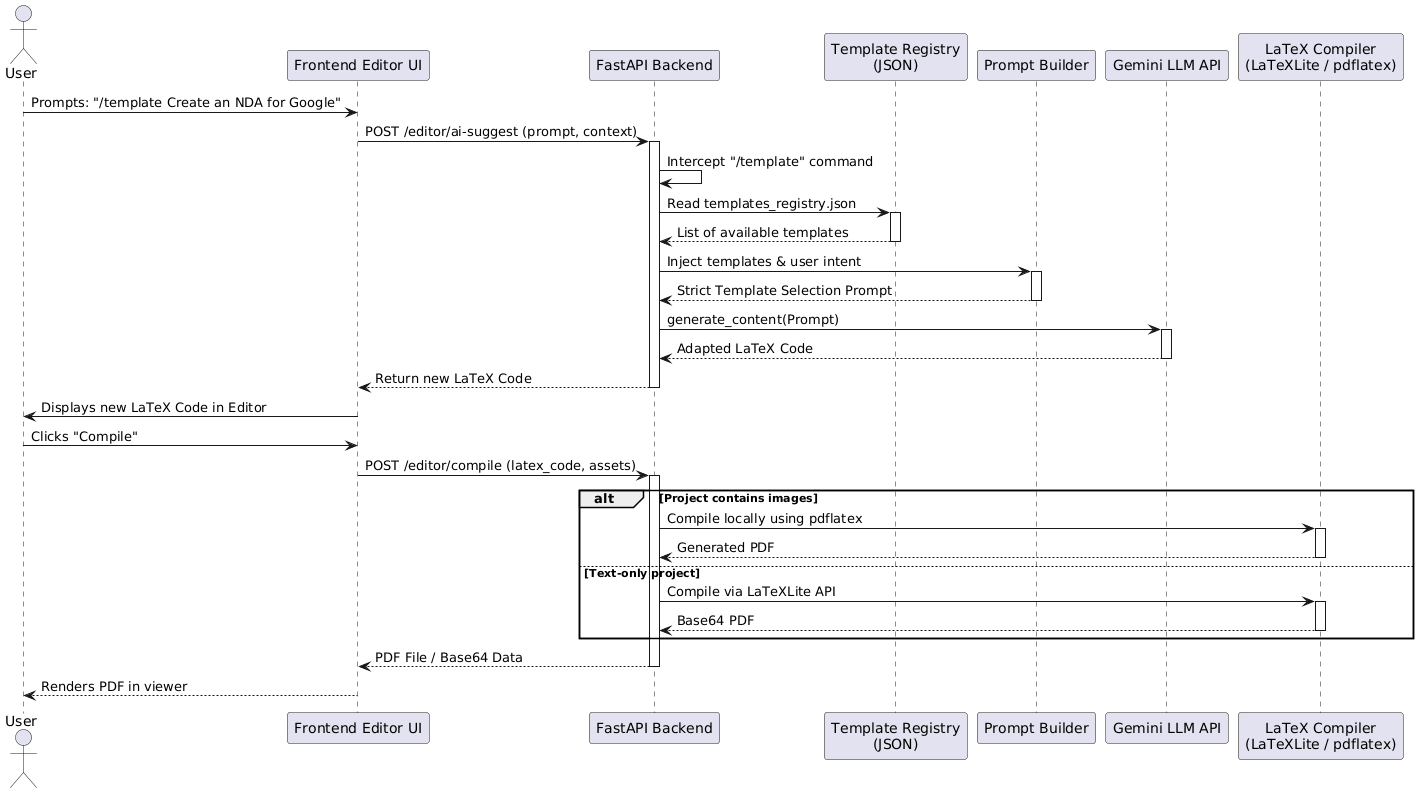
\includegraphics[width=0.9\textwidth, keepaspectratio]{Figures/seq_doc_generation.png}
    }{
        \framebox[14cm]{\rule{0pt}{7cm} \textbf{Missing Image: Figures/seq\_doc\_generation.png}}
    }
    \caption{Sequence Diagram of AI-Assisted Document Generation and Hybrid Compilation.}
    \label{fig:seq_generation}
\end{figure}

\newpage

\section{Database Architecture and Optimization}

\subsection{Class Diagram (Entity-Relationship Model)}
The Class Diagram serves as the foundational architectural blueprint for the PostgreSQL database. It illustrates the core entities—such as Users, Chat Sessions, Messages, and Documents—along with their precise attributes, primary keys, foreign keys, and relational multiplicities, ensuring a highly normalized and structurally sound data model.

\begin{figure}[H]
    \centering
    \IfFileExists{Figures/class_database.png}{
        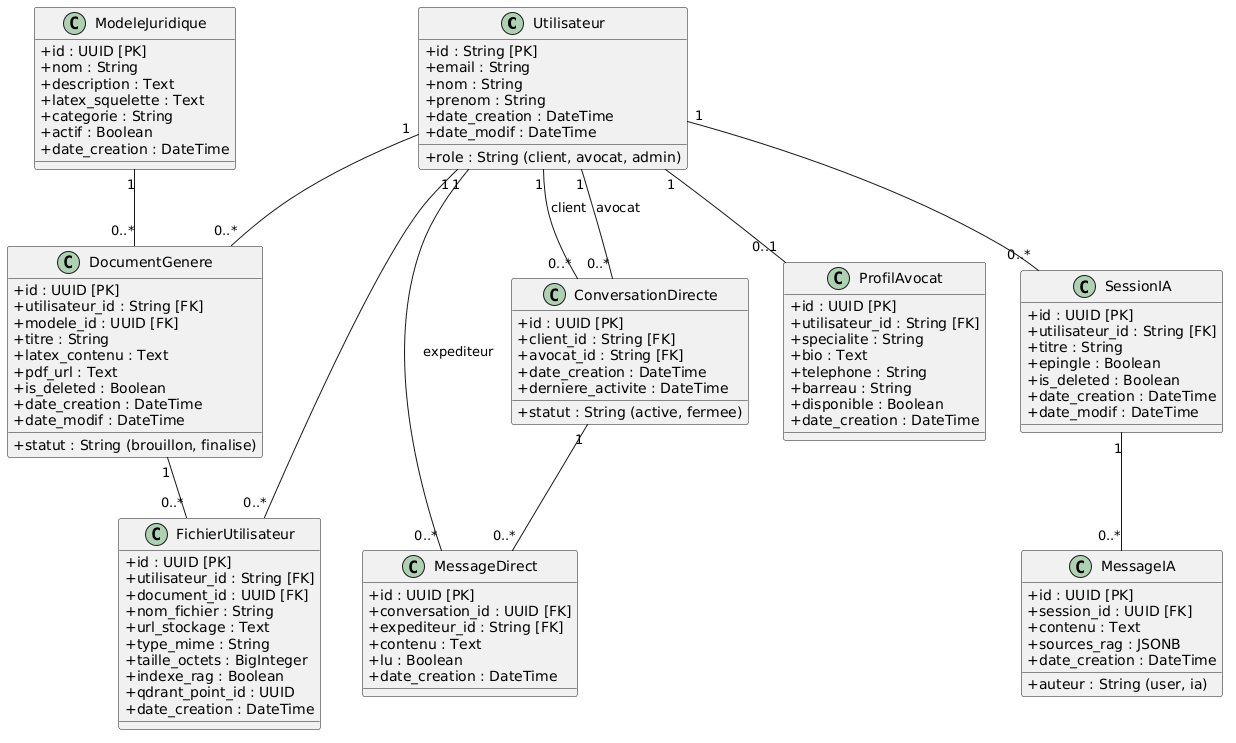
\includegraphics[width=0.9\textwidth, keepaspectratio]{Figures/class_database.png}
    }{
        \framebox[14cm]{\rule{0pt}{7cm} \textbf{Missing Image: Figures/class\_database.png}}
    }
    \caption{UML Class Diagram representing the PostgreSQL Relational Database Schema.}
    \label{fig:class_diagram}
\end{figure}

\subsection{Database Optimization Strategies}
To guarantee enterprise-grade performance, absolute data integrity, and secure tenant isolation, advanced structural optimizations were implemented directly within the PostgreSQL engine.

\begin{itemize}
    \item \textbf{Advanced Indexing Strategies:} To minimize latency on high-volume queries, several complex index structures were deployed:
    \begin{itemize}
        \item \textit{Partial \& Compound Indexes:} Deployed \texttt{idx\_sessions\_active} to index strictly active sessions while pre-sorting by \texttt{date\_modif DESC}, enabling instantaneous UI rendering.
        \item \textit{Foreign Key Indexing:} Explicitly indexed all relational foreign keys to completely eliminate full-table scans during heavy \texttt{JOIN} operations.
        \item \textit{GIN Indexing:} Applied Generalized Inverted Indexes (GIN) to RAG metadata, facilitating rapid semantic searches within JSONB payloads without requiring deserialization.
    \end{itemize}
    
    \item \textbf{PL/pgSQL Triggers \& Automation:} A custom PL/pgSQL function coupled with \texttt{BEFORE UPDATE} triggers autonomously manages all operational timestamps (e.g., dynamically setting \texttt{date\_modif} to \texttt{now()}). This ensures absolute chronological integrity and significantly reduces application-layer boilerplate logic.
    
    \item \textbf{Data Integrity \& Constraints:} Rigorous relational constraints prevent orphaned data anomalies and corrupted system states:
    \begin{itemize}
        \item \textit{Cascading Deletes (\texttt{ON DELETE CASCADE}):} All child dependencies are strictly bound to parent identifiers, ensuring pristine deletions in a single, atomic transaction.
        \item \textit{Check Constraints (\texttt{CHECK}):} Constrained vocabularies (e.g., user roles and document statuses) are strictly enforced directly on columns, rejecting malformed strings before they can corrupt the database.
    \end{itemize}
    
    \item \textbf{Aggregated Views:} A materialized SQL View (\texttt{v\_dashboard\_utilisateur}) was engineered to pre-calculate complex, heavy aggregations (such as session volumes, document counts, and RAG ingestion stats) in a single pass. This unlocks instantaneous analytics retrieval for the Dashboard API without incurring the severe performance penalties of real-time \texttt{COUNT} operations.
\end{itemize}

\section*{Conclusion}
This chapter has established a comprehensive blueprint for the platform by systematically detailing the functional, non-functional, and systemic requirements. By explicitly outlining the user interface paradigms, RAG and LLM integrations, strict performance benchmarks, and robust database optimizations, we have defined the exact technical criteria necessary for a successful implementation. These foundational specifications serve as the definitive reference guiding the software development phases discussed in subsequent chapters.

\pagebreak

\chapter{Technology Overview and Justification}
\label{chap:Technology_Overview}

\section*{Introduction}
This chapter provides an in-depth overview of the frontend, backend, and AI technologies chosen for the development of our GenAI-powered LegalTech system. Each tool and framework was meticulously selected based on its performance, scalability, ease of integration, and ability to meet the project's specific architectural requirements. The following sections explore the functional overview of these technologies and the rationale behind their implementation in our architecture, from interactive user interfaces to advanced Retrieval-Augmented Generation (RAG) pipelines.

\newpage

\section{Frontend Technologies}

\subsection{React.js}
React.js is a declarative, component-based JavaScript library maintained by Meta, used extensively for building highly interactive user interfaces and Single Page Applications (SPAs).

\begin{figure}[H]
    \centering
    \IfFileExists{Figures/react.png}{
        
\includegraphics[width=0.2\textwidth]{Figures/react.png}
    }{
        \framebox[4cm]{\rule{0pt}{2cm} \textbf{react.png}}
    }
    \caption{React Logo}
\end{figure}

\textbf{Why it was used:} React was chosen to build the dynamic, modular interfaces of the platform—specifically the split-screen LaTeX editor, the real-time chat interface, and the interactive document management system. Its component-based state management ensures a smooth, application-like user experience without disruptive page reloads.

\subsection{Vite}
Vite is a modern frontend build tool and development server that provides instantaneous Hot Module Replacement (HMR) and highly optimized production builds.

\begin{figure}[H]
    \centering
    \IfFileExists{Figures/vite.png}{
        
\includegraphics[width=0.2\textwidth]{Figures/vite.png}
    }{
        \framebox[4cm]{\rule{0pt}{2cm} \textbf{vite.png}}
    }
    \caption{Vite Logo}
\end{figure}

\textbf{Why it was used:} It drastically accelerates frontend development time compared to older bundlers (like Webpack). Vite ensures that the final deployed application is minified, highly performant, and lightweight, which is critical for modern web applications.

\subsection{Axios}
Axios is a robust, promise-based HTTP client for JavaScript that operates seamlessly within the browser. It provides a clean, easily configurable API for executing asynchronous network requests and handling responses.

\begin{figure}[H]
    \centering
    \IfFileExists{Figures/axios.png}{
        
\includegraphics[width=0.3\textwidth]{Figures/axios.png}
    }{
        \framebox[5cm]{\rule{0pt}{2cm} \textbf{axios.png}}
    }
    \caption{Axios Logo}
\end{figure}

\textbf{Why it was used:} Axios was selected to serve as the critical communication bridge between the React frontend and the FastAPI backend. It was specifically implemented to handle asynchronous REST API calls, automatically manage JSON data transformation, and utilize request interceptors to securely inject Clerk authentication tokens into HTTP headers. This ensures that all data exchange—from real-time chat prompts to heavy document uploads—remains secure, stable, and highly reliable across the platform.

\subsection{Clerk}
Clerk is a comprehensive Identity and Access Management (IAM) platform built for modern web applications, providing drop-in authentication components and secure session management.

\begin{figure}[H]
    \centering
    \IfFileExists{Figures/clerk.png}{
        
\includegraphics[width=0.2\textwidth]{Figures/clerk.png}
    }{
        \framebox[4cm]{\rule{0pt}{2cm} \textbf{clerk.png}}
    }
    \caption{Clerk Logo}
\end{figure}

\textbf{Why it was used:} Clerk was implemented to guarantee enterprise-grade security for user accounts. It handles login, registration, and token generation effortlessly, ensuring that sensitive legal data, chat histories, and uploaded files are strictly isolated and protected per user.

\subsection{Lucide React \& React Markdown}
Lucide is a clean, modern iconography library, while React Markdown is a component used to safely parse and render Markdown syntax directly into HTML elements.

\begin{figure}[H]
    \centering
    \IfFileExists{Figures/lucide_markdown.png}{
        
\includegraphics[width=0.3\textwidth]{Figures/lucide_markdown.png}
    }{
        \framebox[5cm]{\rule{0pt}{2cm} \textbf{lucide\_markdown.png}}
    }
    \caption{Lucide and Markdown Logos}
\end{figure}

\textbf{Why it was used:} Lucide provides the professional visual cues (folder icons, chat icons) across the platform. React Markdown is absolutely critical for rendering the raw mathematical tables, bold text, and structured lists generated by the AI into a highly readable, Notion-style chat interface.


\section{Backend Infrastructure}

\subsection{FastAPI}
FastAPI is a modern, incredibly fast web framework for building APIs with Python. It is based on standard Python type hints and native asynchronous programming.

\begin{figure}[H]
    \centering
    \IfFileExists{Figures/fastapi.png}{
        
\includegraphics[width=0.3\textwidth]{Figures/fastapi.png}
    }{
        \framebox[5cm]{\rule{0pt}{2cm} \textbf{fastapi.png}}
    }
    \caption{FastAPI Logo}
\end{figure}

\textbf{Why it was used:} Selected as the core backend engine due to its exceptional performance and native asynchronous (\texttt{async/await}) capabilities. This is vital for a platform that must simultaneously juggle non-blocking database queries and long-running AI generation requests without freezing the server.

\subsection{PostgreSQL}
PostgreSQL is an advanced, open-source object-relational database system globally recognized for its robust feature set, reliability, and strict data integrity constraints.

\begin{figure}[H]
    \centering
    \IfFileExists{Figures/postgresql.png}{
        
\includegraphics[width=0.2\textwidth]{Figures/postgresql.png}
    }{
        \framebox[4cm]{\rule{0pt}{2cm} \textbf{postgresql.png}}
    }
    \caption{PostgreSQL Logo}
\end{figure}

\textbf{Why it was used:} PostgreSQL acts as the absolute source of truth for the platform. It reliably stores, links, and indexes all relational metadata, including user profiles, session histories, chat logs, virtual folder hierarchies, and LaTeX templates.

\subsection{SQLAlchemy \& Asyncpg}
SQLAlchemy is a comprehensive Python SQL toolkit and Object Relational Mapper (ORM). Asyncpg is a high-performance, asynchronous database driver built specifically for PostgreSQL.

\begin{figure}[H]
    \centering
    \IfFileExists{Figures/sqlalchemy.png}{
        \includegraphics[width=0.3\textwidth]{Figures/sqlalchemy.png}
    }{
        \framebox[5cm]{\rule{0pt}{2cm} \textbf{sqlalchemy.png}}
    }
    \caption{SQLAlchemy Logo}
\end{figure}

\textbf{Why it was used:} SQLAlchemy securely maps Python objects to database tables, preventing SQL injection attacks. The \texttt{asyncpg} driver ensures that high-volume database read and write operations never block the main FastAPI web server thread.


\section{AI \& Retrieval-Augmented Generation (RAG)}

\subsection{ChromaDB}
ChromaDB is an open-source, embedding-native vector database designed specifically to store, index, and query high-dimensional mathematical vectors.

\begin{figure}[H]
    \centering
    \IfFileExists{Figures/chromadb.png}{
        \includegraphics[width=0.3\textwidth]{Figures/chromadb.png}
    }{
        \framebox[5cm]{\rule{0pt}{2cm} \textbf{chromadb.png}}
    }
    \caption{ChromaDB Logo}
\end{figure}

\textbf{Why it was used:} It serves as the core retrieval engine for our RAG pipeline. ChromaDB indexes the semantic chunks of the Moroccan legal corpus, enabling millisecond-latency similarity searches to instantly find the exact legal clauses relevant to a user's question.

\subsection{Google Gemini API (Gemini 2.5 Flash)}
Gemini 2.5 Flash is a state-of-the-art multimodal generative AI model developed by Google, renowned for its massive context window and rapid inference capabilities.

\begin{figure}[H]
    \centering
    \IfFileExists{Figures/gemini.png}{
        
\includegraphics[width=0.3\textwidth]{Figures/gemini.png}
    }{
        \framebox[5cm]{\rule{0pt}{2cm} \textbf{gemini.png}}
    }
    \caption{Google Gemini Logo}
\end{figure}

\textbf{Why it was used:} It acts as the primary cognitive engine of the legal assistant. Gemini reasons over retrieved legal contexts to answer questions, analyzes live user-uploaded PDFs natively, and autonomously adapts boilerplate LaTeX templates into highly customized legal contracts.

\subsection{OpenAI API (GPT-4o Vision)}
GPT-4o is a highly advanced multimodal AI model capable of profound visual reasoning and exceptionally accurate Optical Character Recognition (OCR).

\begin{figure}[H]
    \centering
    \IfFileExists{Figures/openai.png}{
        
\includegraphics[width=0.2\textwidth]{Figures/openai.png}
    }{
        \framebox[4cm]{\rule{0pt}{2cm} \textbf{openai.png}}
    }
    \caption{OpenAI Logo}
\end{figure}

\textbf{Why it was used:} Utilized exclusively in the offline ingestion pipeline to bypass the limitations of traditional OCR. It intelligently "reads" scanned Moroccan legal documents and accurately flattens complex visual elements (like matrices, stamps, and tables) into clean, indexable text.

\subsection{Sentence-Transformers (BAAI/bge-m3)}
BAAI/bge-m3 is an advanced open-source machine learning framework and embedding model used to compute dense, high-dimensional vector representations of text strings.

\begin{figure}[H]
    \centering
    \IfFileExists{Figures/bge_m3.png}{
        
\includegraphics[width=0.3\textwidth]{Figures/bge_m3.png}
    }{
        \framebox[5cm]{\rule{0pt}{2cm} \textbf{bge\_m3.png}}
    }
    \caption{BAAI BGE-M3 Model}
\end{figure}

\textbf{Why it was used:} Chosen specifically for its state-of-the-art multilingual capabilities. It accurately translates Arabic and French legal texts into mathematical vectors, heavily optimizing the semantic matching process for the Moroccan legal domain.

\subsection{FlagEmbedding (BGE-Reranker)}
The BGE-Reranker is a Cross-Encoder neural network that evaluates pairs of texts (a user query and a retrieved document chunk) to output a highly accurate semantic relevance score.


\textbf{Why it was used:} Implemented as the crucial "second stage" of the retrieval pipeline. It drastically reduces AI hallucinations by re-evaluating and filtering the initial broad vector search down to the absolute most precise and contextually relevant chunks before passing them to the LLM.


\section{Utilities \& Document Processing}

\subsection{PyMuPDF}
PyMuPDF is a high-performance Python library used for rapid document rendering, PDF parsing, and raw text extraction.

\begin{figure}[H]
    \centering
    \IfFileExists{Figures/pymupdf.png}{
        \includegraphics[width=0.3\textwidth]{Figures/pymupdf.png}
    }{
        \framebox[5cm]{\rule{0pt}{2cm} \textbf{pymupdf.png}}
    }
    \caption{PyMuPDF Logo}
\end{figure}

\textbf{Why it was used:} Implemented for instantaneous text extraction from digitally native PDFs uploaded by users in the live chat. It allows the system to bypass the database ingestion process and inject full document contents directly into the LLM's context window on the fly.

\subsection{LaTeXLite API \& MiKTeX}
LaTeXLite is a cloud-based LaTeX compilation service, while MiKTeX is a standard, robust local TeX distribution engine for Windows environments.

\begin{figure}[H]
    \centering
    % First Image
    \begin{minipage}{0.25\textwidth}
        \centering
        \IfFileExists{Figures/latex.png}{
            
\includegraphics[width=\linewidth]{Figures/latex.png}
        }{
            \framebox[4cm]{\rule{0pt}{2cm} \textbf{latex.png}}
        }
    \end{minipage}% Notice we removed \hfill here
    \hspace{1cm} % <--- This controls the gap between the images. Change 1cm to whatever you prefer!
    % Second Image
    \begin{minipage}{0.25\textwidth}
        \centering
        \IfFileExists{Figures/latex1.png}{
            
\includegraphics[width=\linewidth]{Figures/latex1.png}
        }{
            \framebox[4cm]{\rule{0pt}{2cm} \textbf{latex1.png}}
        }
    \end{minipage}
    
    \caption{LaTeX Compilation Tools}
\end{figure}
\textbf{Why it was used:} Deployed in a dynamic, hybrid configuration to render generated LaTeX code into printable PDFs. The cloud API handles ultra-fast, text-only compilations, while the local MiKTeX engine acts as a robust fallback to compile complex legal documents containing custom user images (like company logos or signatures).
\subsection{uv (Python Package Manager)}
uv is an extremely fast Python package and project manager, written in Rust, designed as a modern, high-performance replacement for standard pip.


\textbf{Why it was used:} Selected to drastically accelerate the installation of massive Machine Learning dependencies (like PyTorch and Transformers) and to ensure strict, reproducible virtual environments across development and production machines.


\section{Development and Collaboration Tools}

\subsection{Postman}
Postman is a comprehensive API development and testing platform that simplifies the process of building, documenting, and testing RESTful web services.

\begin{figure}[H]
    \centering
    \IfFileExists{Figures/postman.png}{
        
\includegraphics[width=0.2\textwidth]{Figures/postman.png}
    }{
        \framebox[4cm]{\rule{0pt}{2cm} \textbf{postman.png}}
    }
    \caption{Postman Logo}
\end{figure}

\textbf{Why it was used:} Postman was utilized to rigorously test and debug the FastAPI endpoints independently from the frontend. It allowed the team to simulate client requests, verify JSON responses, and ensure that complex interactions—such as multimodal file uploads and RAG query executions—functioned correctly before full system integration.

\subsection{Git}
Git is a distributed version control system designed to handle everything from small to very large projects with speed, efficiency, and data integrity.

\begin{figure}[H]
    \centering
    \IfFileExists{Figures/git.png}{
        
\includegraphics[width=0.2\textwidth]{Figures/git.png}
    }{
        \framebox[4cm]{\rule{0pt}{2cm} \textbf{git.png}}
    }
    \caption{Git Logo}
\end{figure}

\textbf{Why it was used:} Git was implemented to track changes in the source code during development. It enabled the team to maintain a clean, chronological history of modifications, safely experiment with new features via isolated branching, and manage code stability locally without risking the main project structure.

\subsection{GitHub}
GitHub is a cloud-based platform that hosts Git repositories, offering advanced features for remote collaboration, peer code review, and project management.

\begin{figure}[H]
    \centering
    \IfFileExists{Figures/github.png}{
        
\includegraphics[width=0.2\textwidth]{Figures/github.png}
    }{
        \framebox[4cm]{\rule{0pt}{2cm} \textbf{github.png}}
    }
    \caption{GitHub Logo}
\end{figure}

\textbf{Why it was used:} It served as the central hub for team collaboration. GitHub allowed the team to securely store the codebase online, conduct peer code reviews via Pull Requests, and utilize issue tracking to manage tasks, ensuring a transparent, agile, and synchronized development workflow.

\section*{Conclusion}
In this chapter, we have outlined the rationale behind the selection of the core frameworks, AI models, and infrastructure components integral to our LegalTech platform. Each technology—from React and FastAPI to ChromaDB and Gemini—was carefully chosen to address specific operational needs, such as high-concurrency performance, precise semantic retrieval, and asynchronous processing. By combining robust foundational tools with state-of-the-art generative AI and computer vision models, we have established a highly secure, scalable, and adaptable architecture. This technical stack provides the perfect foundation to support the complex computational and cognitive tasks required to process, analyze, and generate Moroccan legal intelligence.

\pagebreak

\chapter{Architecture Design}
\label{chap:architecture_design}

\section*{Introduction}
This chapter provides a detailed exploration of the system architecture, which is designed to be modular, scalable, and secure. Key components include the integration of Large Language Models (LLMs), the implementation of a highly specialized Retrieval-Augmented Generation (RAG) architecture, modern frontend and backend architecture used, the log systesm used in this project.

\pagebreak

\section{Detailed Component Architecture}

The platform's backend architecture follows a highly decoupled approach using FastAPI. This ensures that services are modular, asynchronous, and scalable.
\subsection{Backend Design}
\begin{itemize}


\item \textbf{Data Management:} Uses PostgreSQL (\texttt{asyncpg}/SQLAlchemy) for highly responsive data storage. It enforces strict tenant isolation via Row-Level Security (RLS), storing user files and projects in dedicated, authenticated directories with zero public exposure.

\item \textbf{System Logging \& Telemetry:} An asynchronous JSON logging system tracks all API, database, and RAG operations. It ensures security by scrubbing sensitive data via Regex, and optimizes storage through nightly \texttt{.gz} compression with an automated 30-day deletion policy.

\IfFileExists{Figures/logArch.png}{
    \begin{figure}[H]
        \centering
        \includegraphics[width=0.8\textwidth]{Figures/logArch.png}
        \caption{Architecture of the Rotating JSON Log System}
        \label{fig:log_system}
    \end{figure}
}{}

\item \textbf{Authentication \& APIs:} \textbf{Clerk} handles secure Identity and Access Management via clerk, which the backend strictly verifies to enforce data ownership. A fully asynchronous FastAPI layer, auto-documented via Swagger, orchestrates all internal routing and external AI integrations (Gemini, OpenAI, LaTeXLite).

\IfFileExists{Figures/backend.png}{
    \begin{figure}[H]
        \centering
        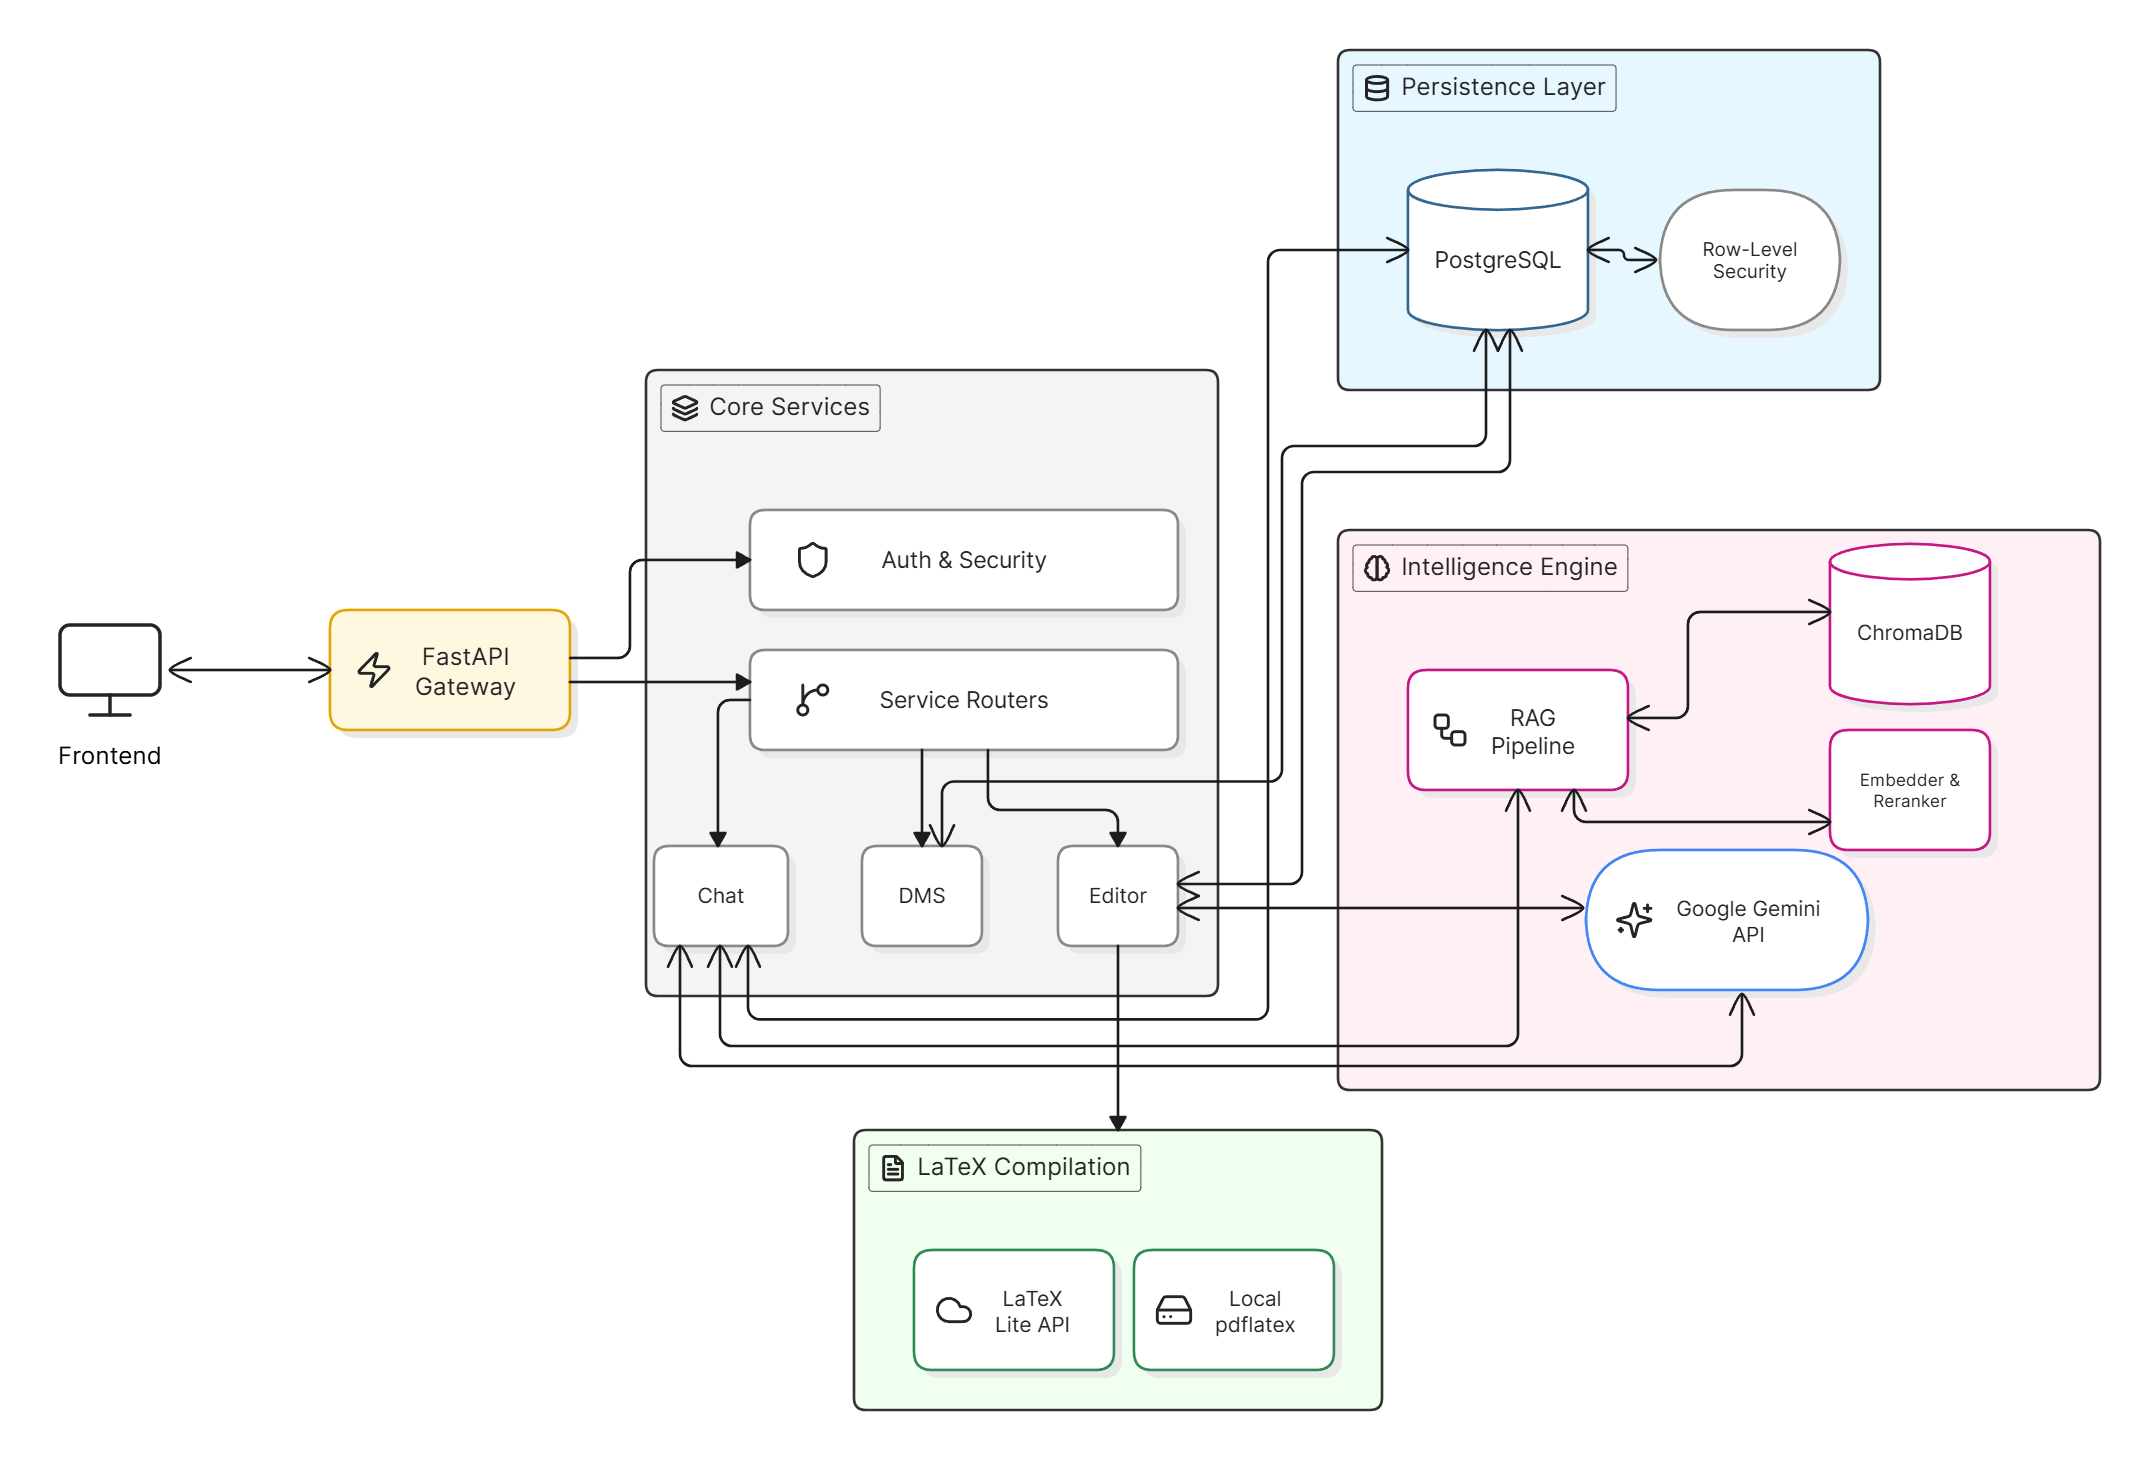
\includegraphics[width=0.8\textwidth]{Figures/backend.png}
        \caption{Detailed Backend Component Architecture}
        \label{fig:backend_arch}
    \end{figure}
}{}
\end{itemize}

\newpage
\section{RAG Architecture \& Intelligence Pipeline}

Our Retrieval-Augmented Generation (RAG) architecture is divided into two distinct, asynchronous phases to maximize accuracy and efficiently handle the morphological complexities of Moroccan legal documents.

\subsection{Phase 1: Offline Ingestion \& Storage}
The ingestion process begins by processing raw legal PDFs through \texttt{PyMuPDF} and \texttt{pdf2image}. These extracted images are routed to a Vision-Language Model (\textbf{GPT-4o Vision}) instructed by a strict, domain-specific prompt. This prompt forces the model to filter out administrative noise (such as repetitive headers, dates, and stamps) and autonomously structure the text using precise XML tags (\texttt{<chunk>} and \texttt{<table>}). 

A custom Python parser then segments this output. The text segments are mathematically embedded using the multilingual \texttt{BAAI/bge-m3} model and indexed securely in a \textbf{ChromaDB} vector store. Crucially, to optimize retrieval and prevent token overflow, only the descriptive titles of tables are embedded, while the full Markdown table structures are preserved securely within the payload metadata.

\subsection{Phase 2: Online Retrieval \& Generation}
During a live chat session, the user's query is intercepted and embedded using the same \texttt{BAAI/bge-m3} model. The system executes a high-speed cosine similarity search against ChromaDB, retrieving the Top 20 most mathematically relevant chunks. 

Because raw vector similarity can lack deep semantic nuance, these 20 chunks are passed through a Cross-Encoder neural network (\texttt{BAAI/bge-reranker-v2-m3}). The reranker evaluates the logical relationship between the query and each chunk, isolating the absolute Top 5 most relevant pieces of context. Finally, this highly refined context is assembled into a strict Arabic system prompt and dispatched to \textbf{Google Gemini 2.5 Flash}, which generates the final, hallucination-free legal response.

\IfFileExists{image.png}{
    \begin{figure}[H]
        \centering
        
\includegraphics[width=0.6\textwidth]{image.png}
        \caption{RAG Pipeline Execution Architecture}
        \label{fig:rag_arch}
    \end{figure}
}{}

\newpage
\section{Frontend Design}

The frontend is a Multiple Page Application (MPA) built using \textbf{React}. It employs a modular component architecture and a clean user interface. the color palette and typography (fonst) are inspired by the \textbf{Ollama} platform, while the conversational interface mirrors the intuitive layout of \textbf{Google Gemini}. Furthermore, the document editing workspace takes structural cues from \textbf{Overleaf} and the \textbf{Antigravity} AI coding tool, paired with a file management system that replicates the seamless, drag-and-drop experience of a native desktop file explorer. 

\subsection{Application Routing Tree (Sitemap)}
The application leverages \texttt{react-router-dom} to manage client-side navigation seamlessly without reloading the browser. The route structure is organized as follows:

\begin{verbatim}
/ (Root)
|-- /sign-in                  -> Authentication Portal (Clerk)
|-- /sign-up                  -> Registration Portal (Clerk)
|-- /                         -> Landing Page (Public overview & features)
|
|-- /chat                     -> Main AI Interface
|   |-- /chat/:id             -> Specific AI Conversation Thread
|
|-- /database                 -> Document Management System (DMS)
|                                (Virtual folders, upload, pagination, sorting)
|
|-- /editor                   -> Workspace for LaTeX Generation
|   |-- /editor/:id           -> Split-Screen Editor (Code / PDF Viewer / AI)
\end{verbatim}

\subsection{UI and Prototyping}

During the initial design phase, we utilized \textbf{Excalidraw} to draft the UI/UX wireframes and conceptualize the platform's layout. The primary objective of these mockups was to bridge the gap between the complex backend architecture and the end-user. By designing an intuitive, accessible, and highly visual interface, we ensure that users can effortlessly leverage all the advanced backend functionalities (such as the RAG pipeline and LaTeX compiler), thereby significantly enhancing the overall user experience.

The following figures illustrate the low-fidelity wireframes created to map out the user journeys across the platform's core modules.

\IfFileExists{Figures/landingPage.png}{
    \begin{figure}[H]
        \centering
        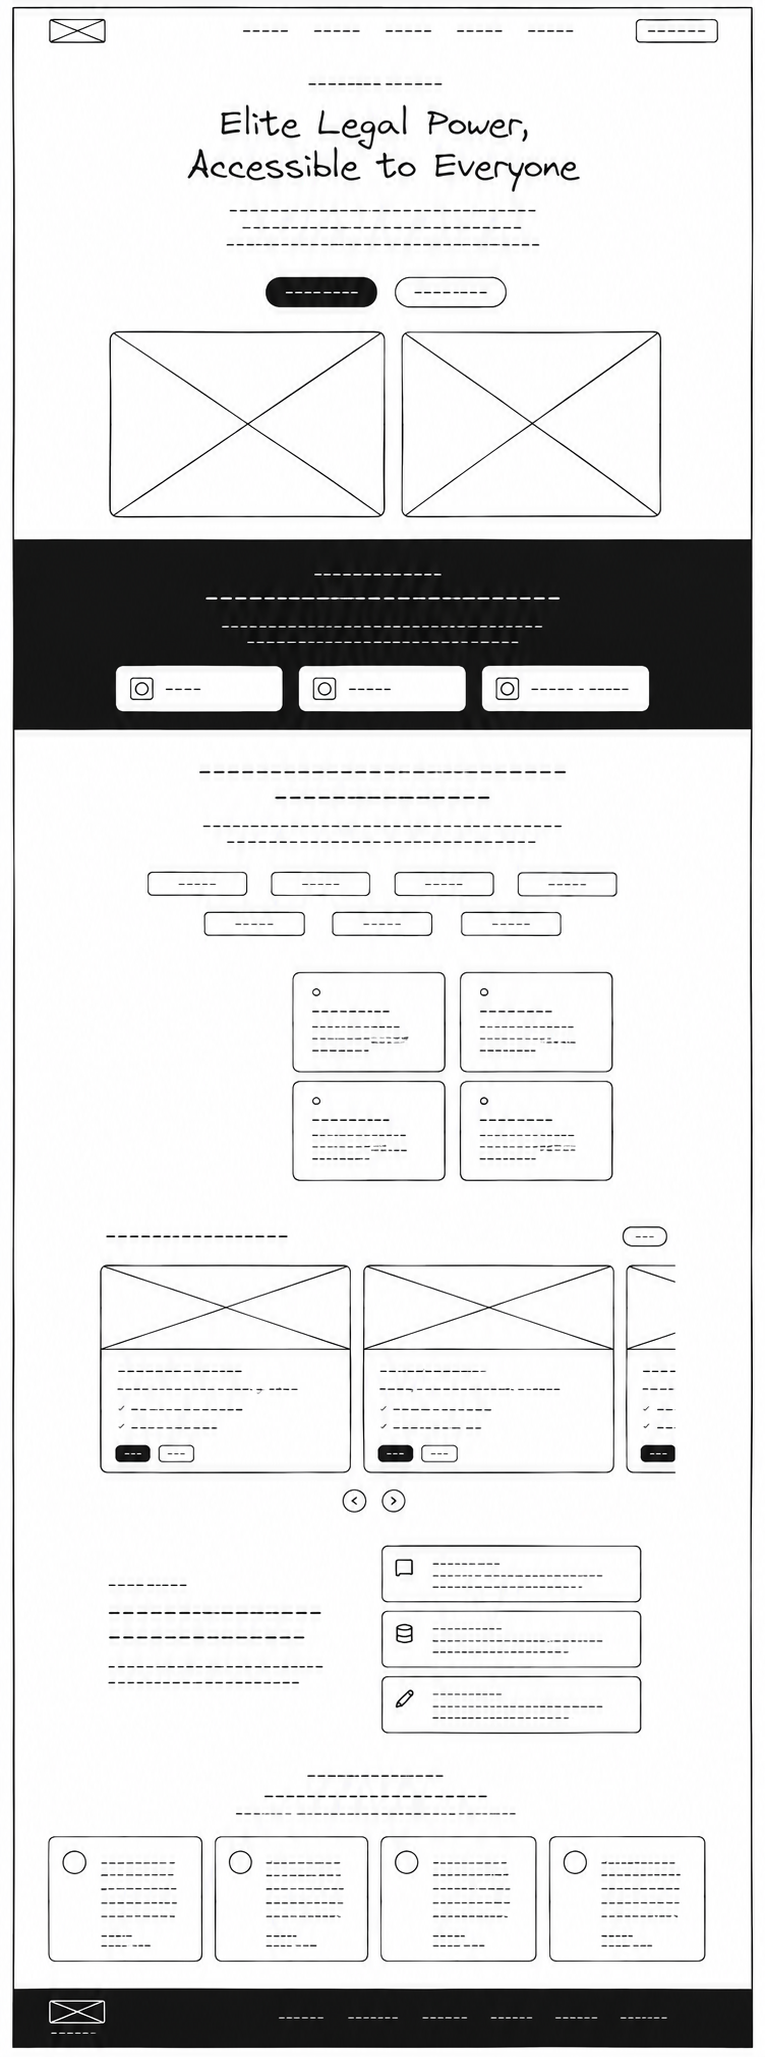
\includegraphics[width=0.55\textwidth]{Figures/landingPage.png}
        \caption{Wireframe mockup of the Public Landing Page}
        \label{fig:wireframe_landing}
    \end{figure}
}{}

\vspace{0.5cm}

\IfFileExists{Figures/chatpage.png}{
    \begin{figure}[H]
        \centering
        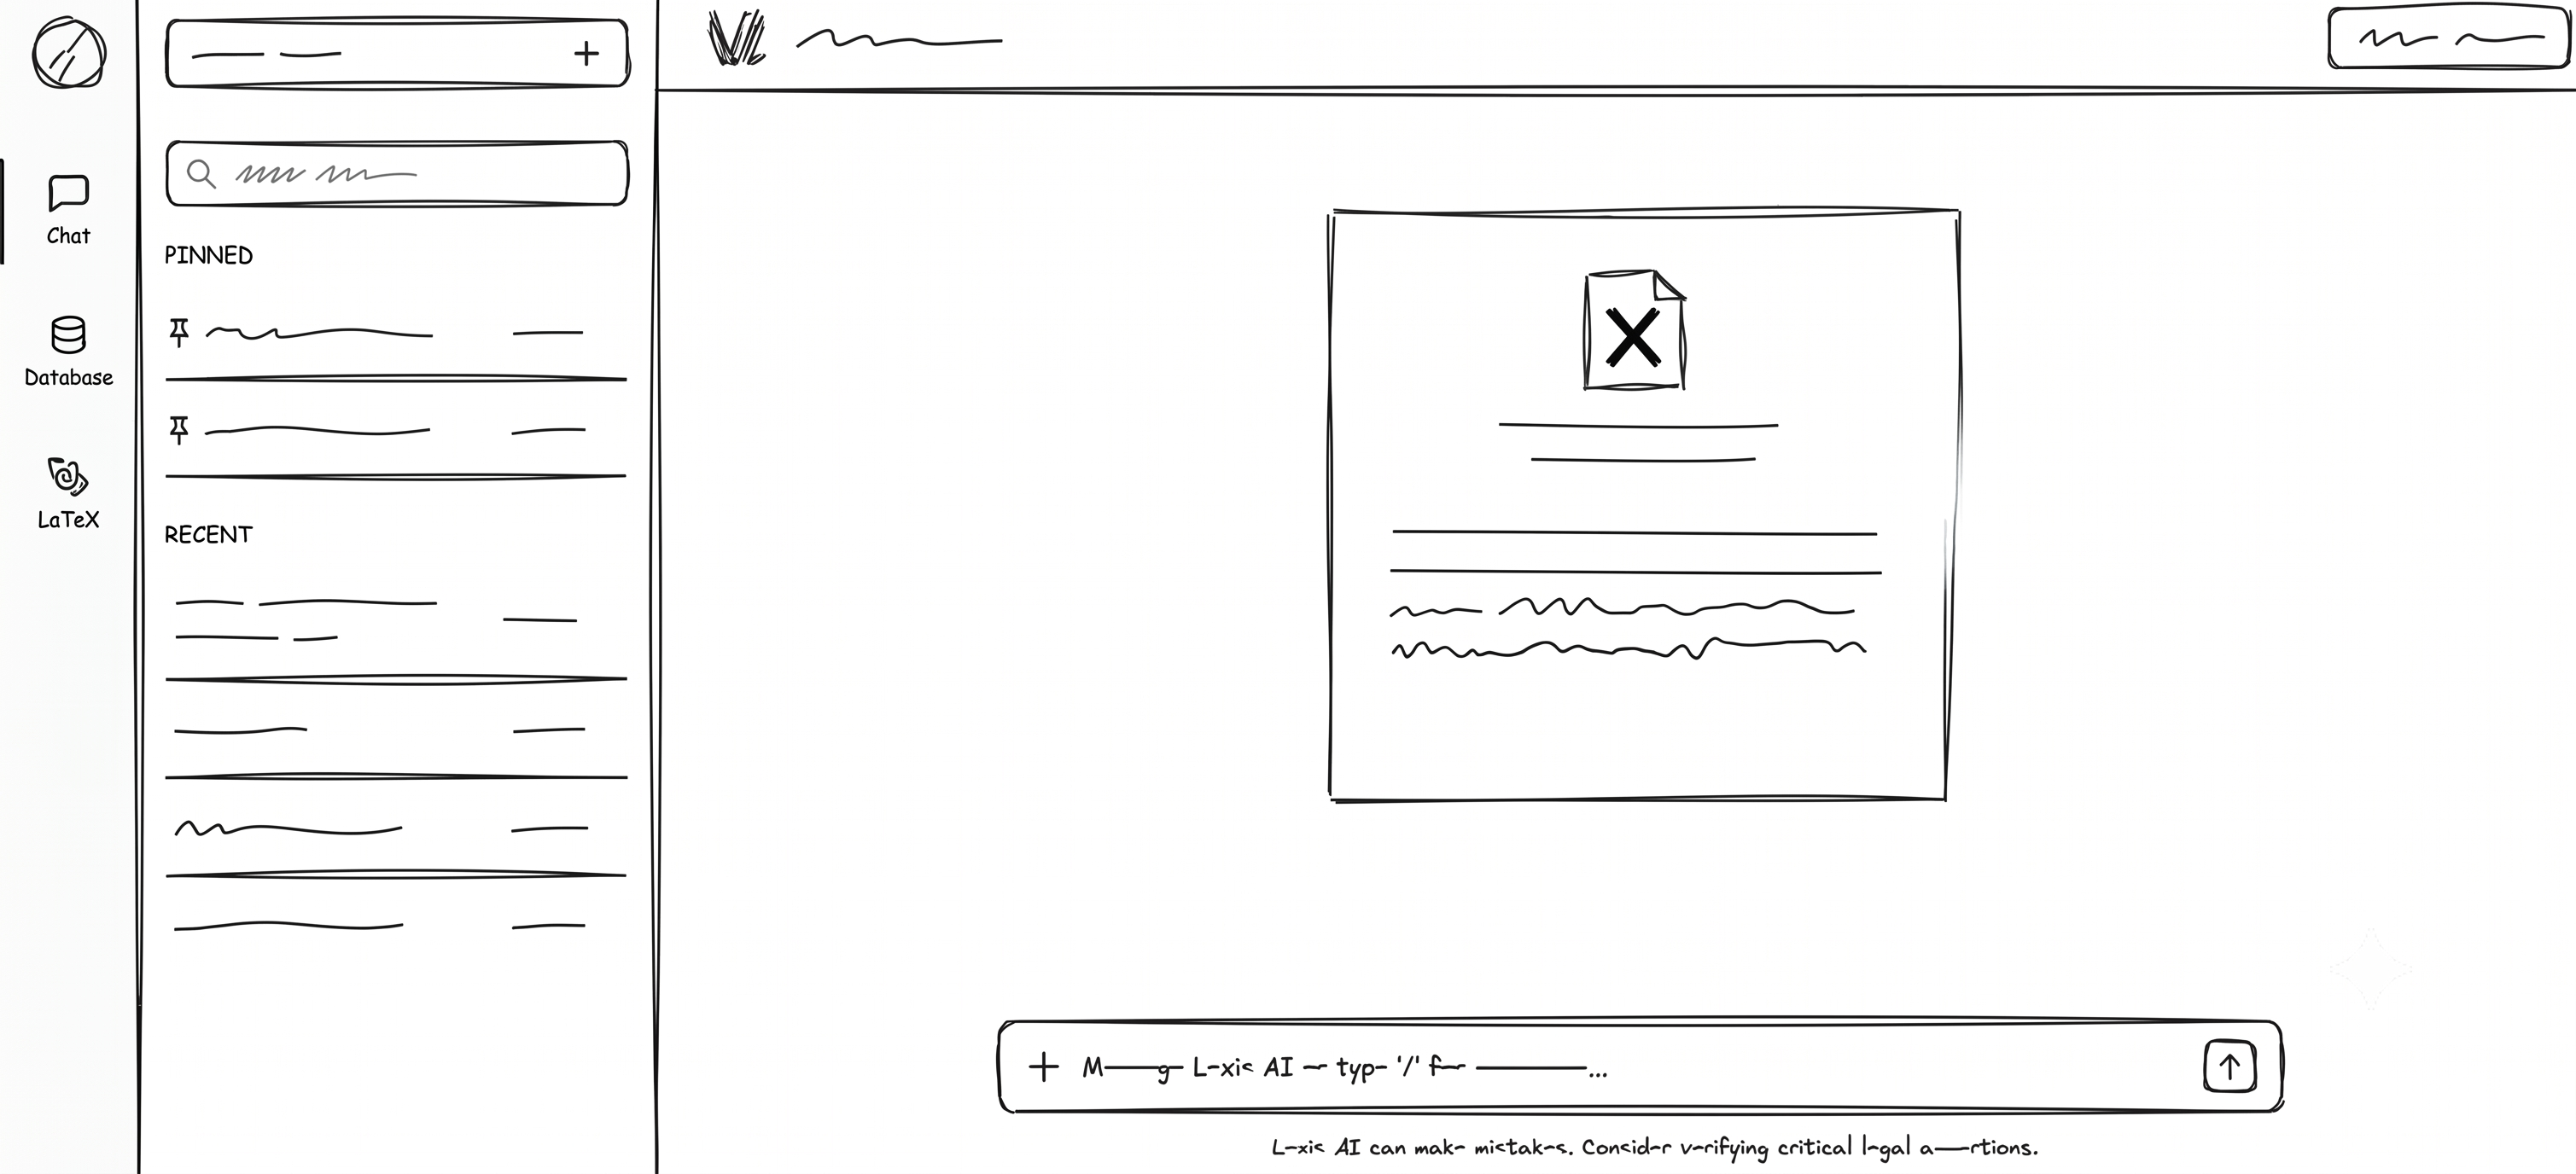
\includegraphics[width=0.9\textwidth]{Figures/chatpage.png}
        \caption{Wireframe mockup of the Main AI Chat Interface}
        \label{fig:wireframe_chat}
    \end{figure}
}{}

\vspace{0.5cm}

\IfFileExists{Figures/latexPage.png}{
    \begin{figure}[H]
        \centering
        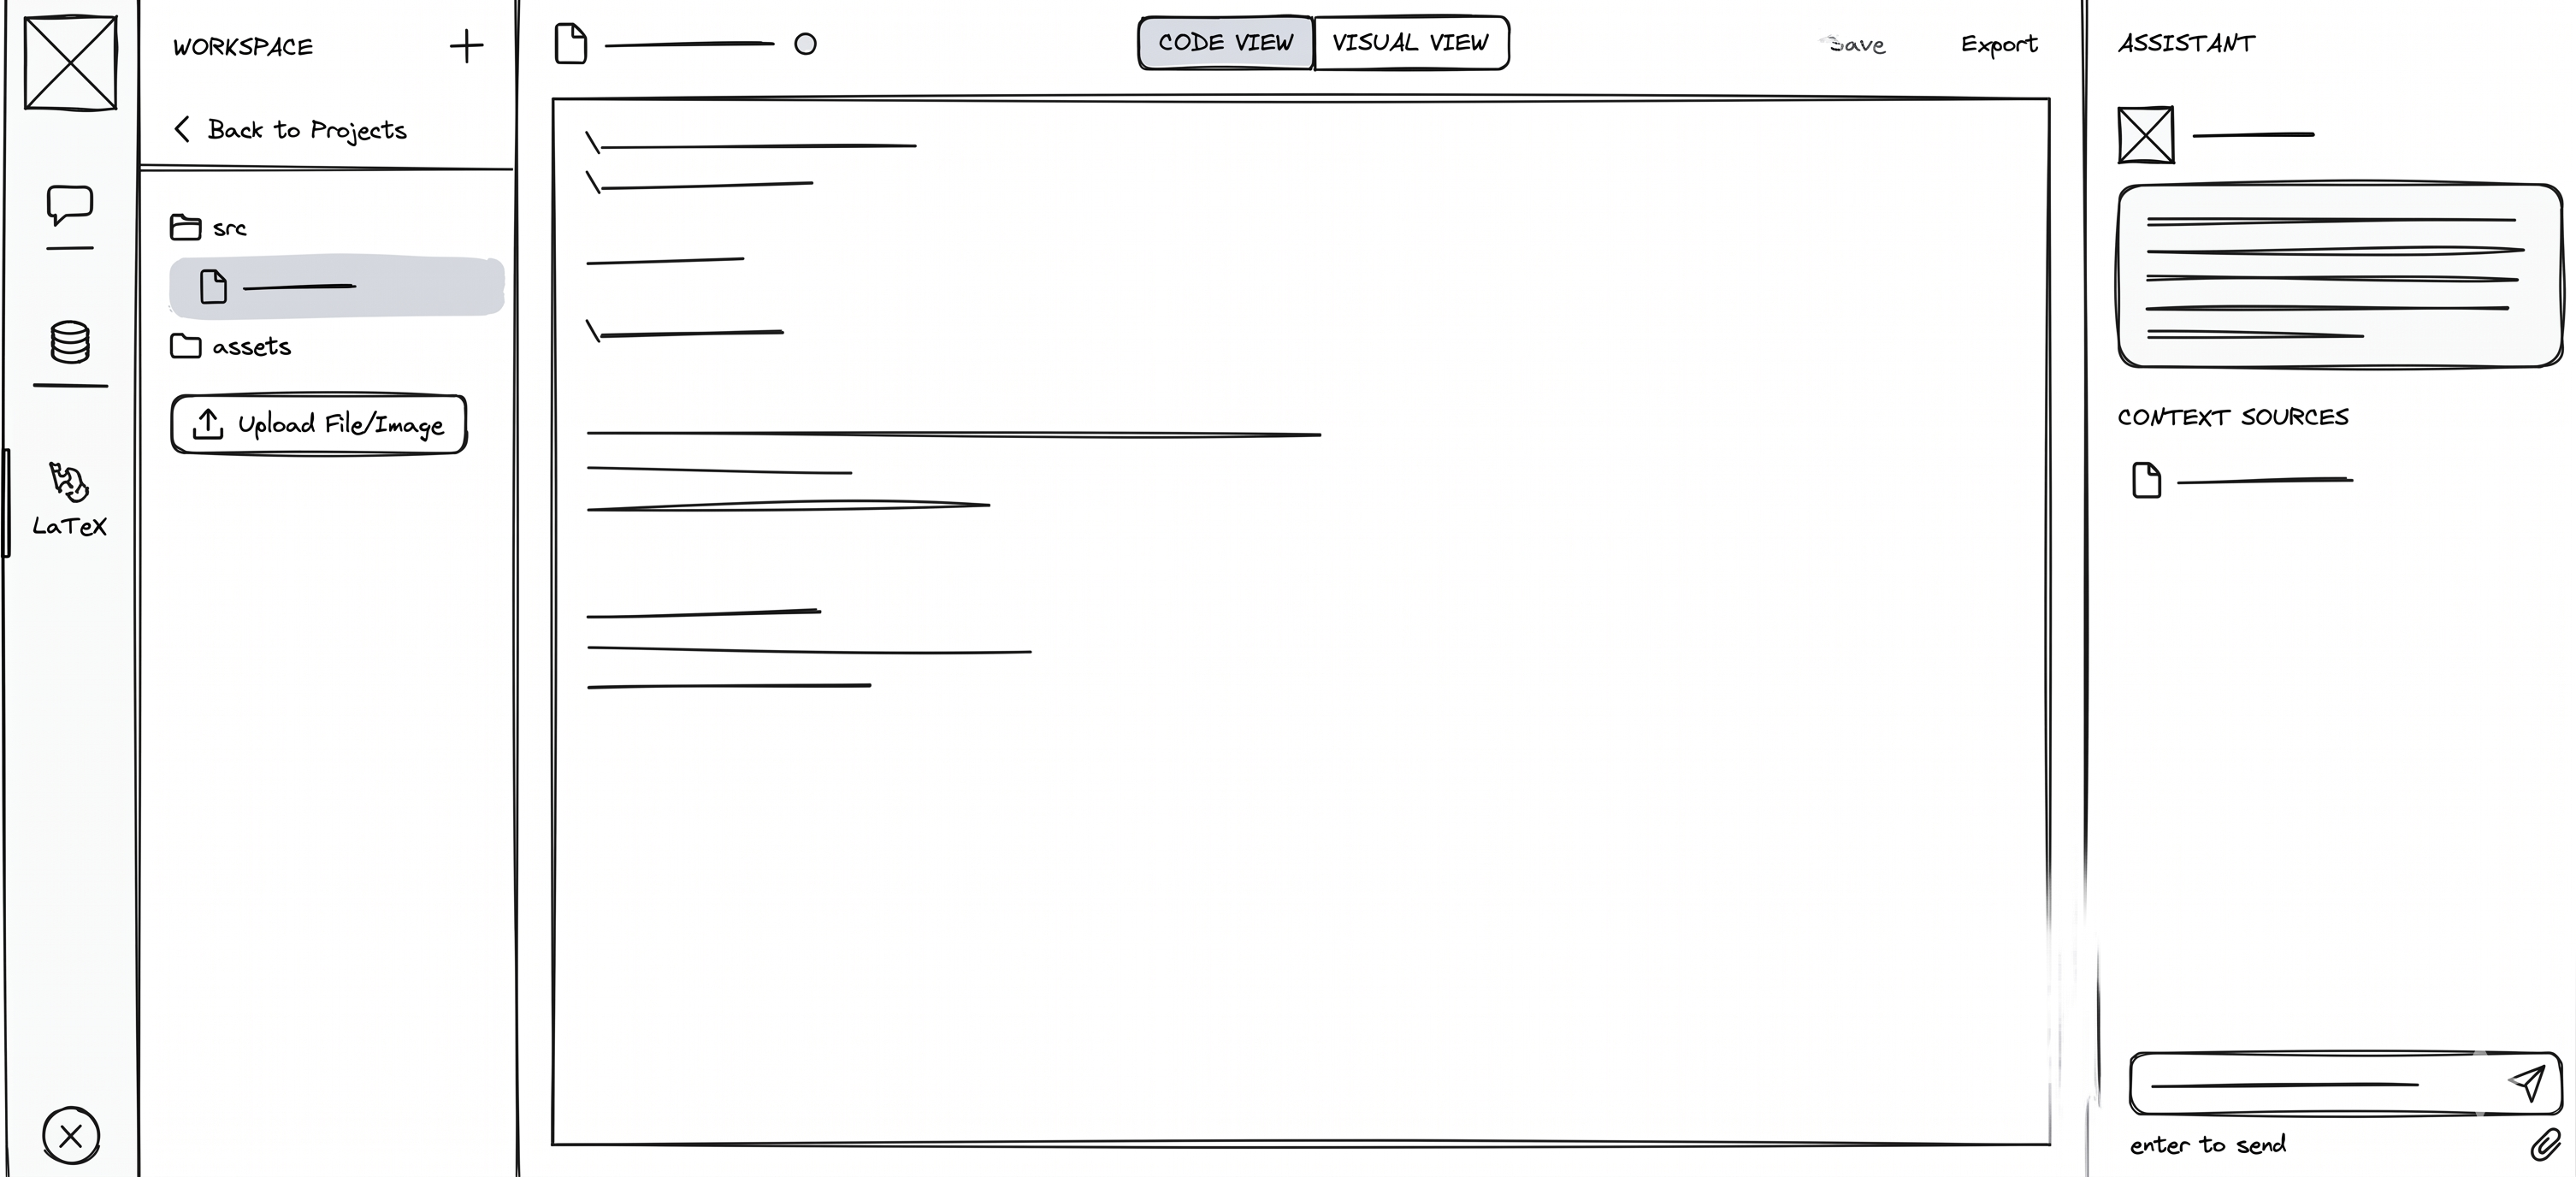
\includegraphics[width=0.9\textwidth]{Figures/latexPage.png}
        \caption{Wireframe mockup of the Split-Screen LaTeX Editor Workspace}
        \label{fig:wireframe_latex}
    \end{figure}
}{}

\vspace{0.5cm}

\IfFileExists{Figures/fileUploads.png}{
    \begin{figure}[H]
        \centering
        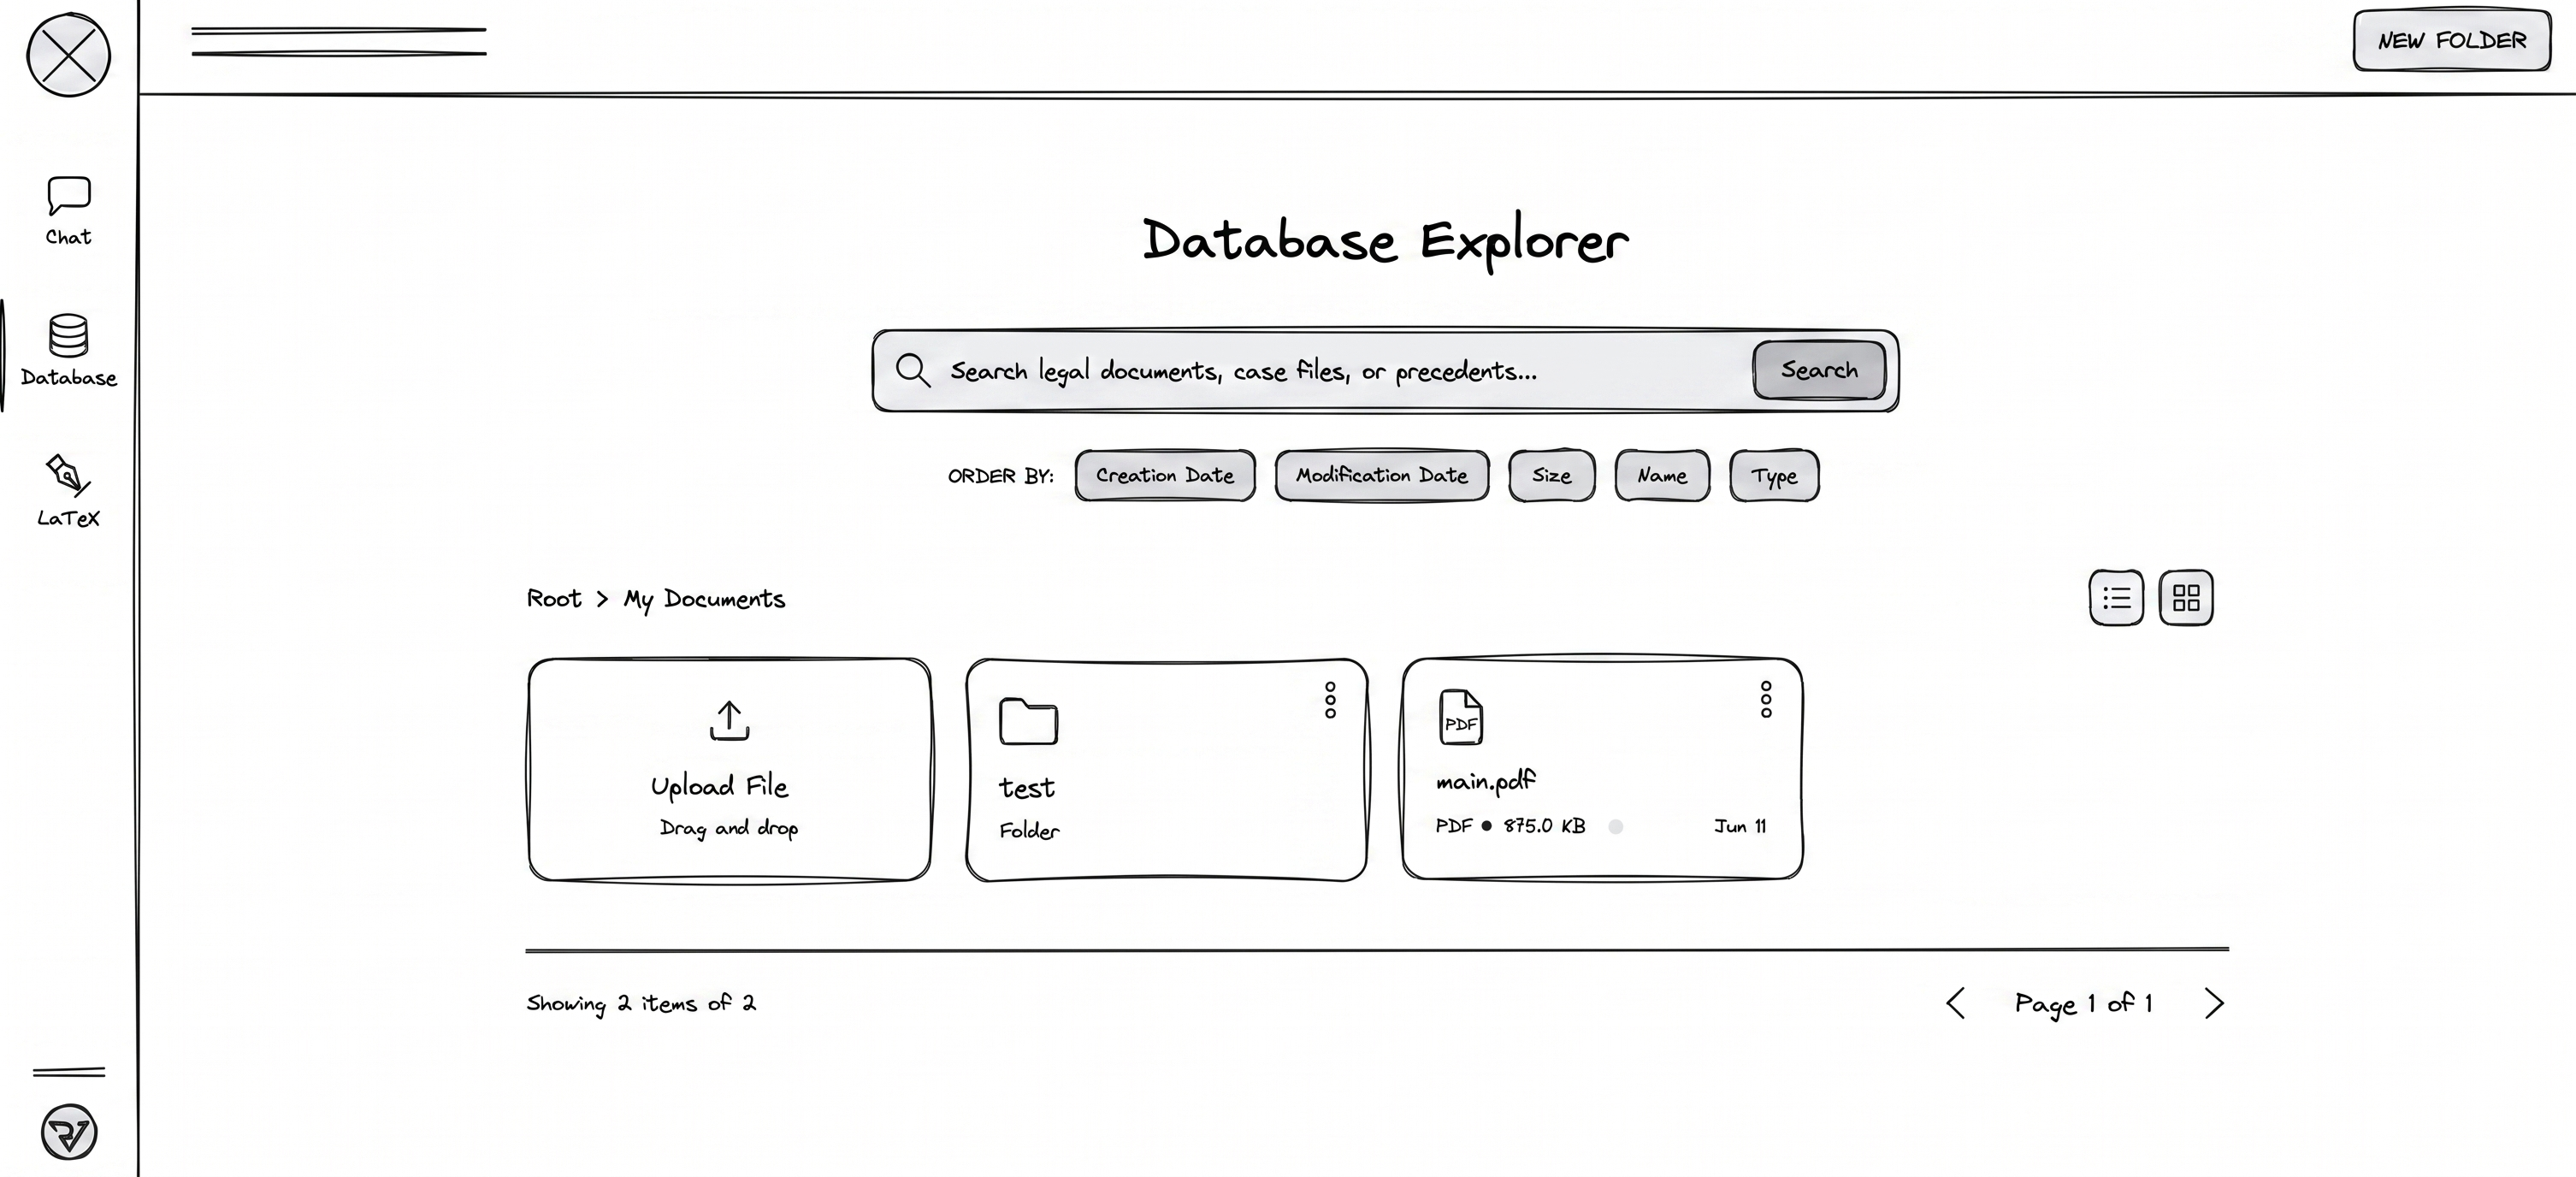
\includegraphics[width=0.9\textwidth]{Figures/fileUploads.png}
        \caption{Wireframe mockup of the Document Management System (Database Explorer)}
        \label{fig:wireframe_files}
    \end{figure}
}{}






\newpage
\section*{Conclusion}
The architecture designed for this platform successfully bridges the gap between complex legal data processing and seamless user interaction. By decoupling the heavy RAG ingestion pipeline from the main web server, implementing a robust custom logging system, and utilizing an asynchronous FastAPI backend paired with a reactive React frontend, the system achieves enterprise-grade stability and performance.


\chapter{Demonstration and Evaluation}
\label{chap:Demonstration_and_Evaluation}

\section*{Introduction}
This chapter transitions the platform from a theoretical architectural framework into a practical, deployed asset. It begins with a comprehensive user roadmap that maps out real-world application workflows. Following this overview, the system's operational modules are demonstrated through an end-to-end user experience narrative, tracing every interactive state from the initial portal arrival to autonomous legal document compilation. Finally, the chapter presents an algorithmic evaluation focused specifically on the performance latency of the FastAPI backend framework and the precision metrics of our multi-query Retrieval-Augmented Generation (RAG) pipeline.

\pagebreak

\section{User Expected Roadmap}
To contextualize the platform's operational flow, this section highlights the sequential journey of a legal professional executing routine case management tasks. The interface seamlessly coordinates these tasks across independent views to transform raw documents into formal outputs:

\begin{enumerate}
    \item \textbf{Ingestion \& Parsing:} Scanned or digital documents are securely uploaded to the system's storage layer, instantly initializing background Optical Character Recognition (OCR) extraction and semantic vectorization pipelines.
    \item \textbf{Data Discovery:} Vectorized records are managed within a unified database explorer, allowing the user to search metadata, filter documents by practice area, or isolate specific context pools.
    \item \textbf{AI Consultation:} Users deploy the chat interface to execute semantic interrogations on their managed database, relying on conversational memory and reranked context to retrieve highly accurate, hallucination-free legal citations.
    \item \textbf{Automated Drafting:} Validated legal research is carried into the workspace composer, where the AI dynamically adapts code templates to compile formal, print-ready PDF documents.
\end{enumerate}

\newpage

\section{Functional Workspace Demonstration}
This section provides an interactive narrative walkthrough, tracking the sequential states of the application as experienced by a legal professional navigating a complete session.

\subsection{Portal Entry and Session Authentication}
Upon accessing the platform, the user is greeted by the Landing Page, which concisely outlines the application's core LegalTech functionalities. From this entry point, they can initiate the authentication process by clicking the "Sign In" or "Get Started" buttons, seamlessly securing their session via the Clerk Identity provider. 

\IfFileExists{Figures/11.png}{
    \begin{figure}[H]
        \centering
        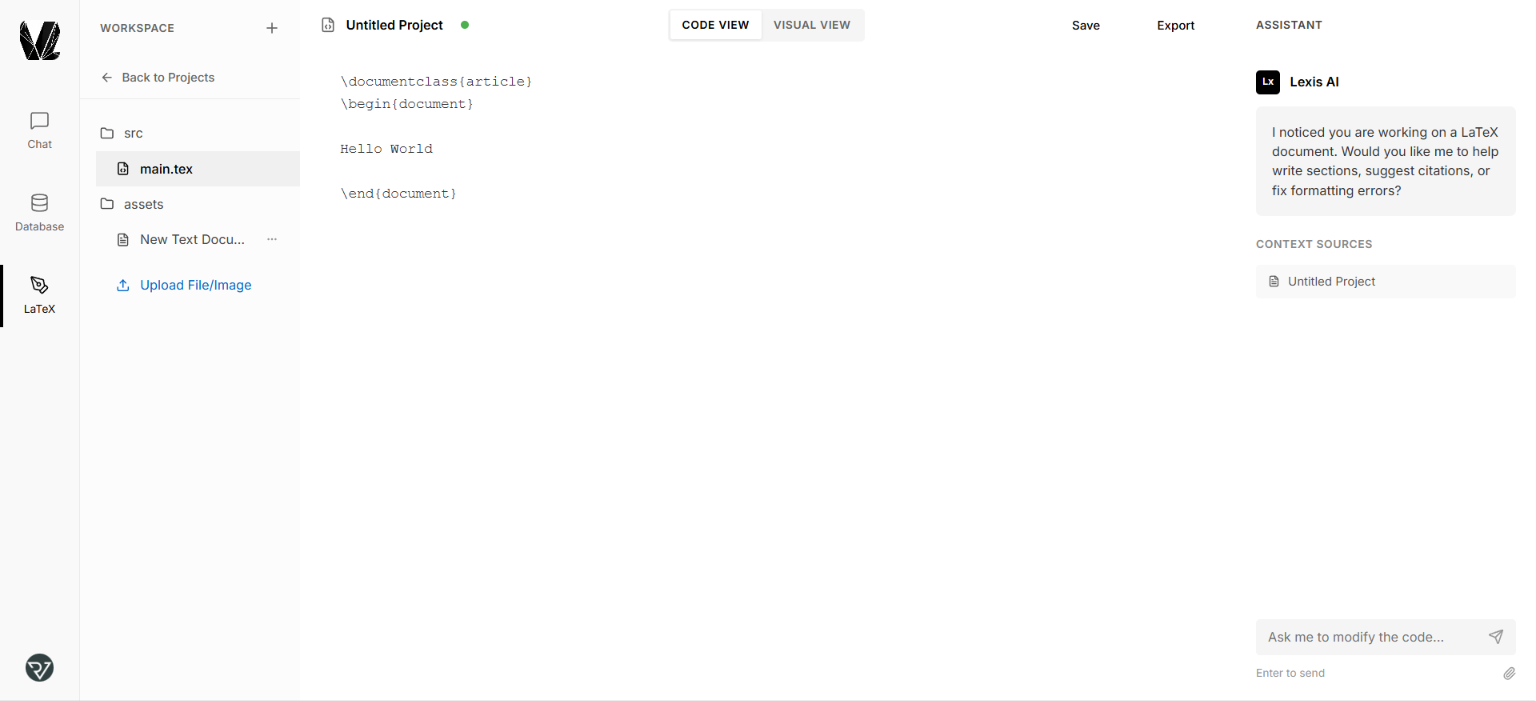
\includegraphics[width=0.85\textwidth, keepaspectratio]{Figures/11.png}
        \caption{Public Landing Page Outlining Core LegalTech Features.}
        \label{fig:demo_landing}
    \end{figure}
}{}

Users are afforded the flexibility to authenticate using standard credentials or third-party OAuth providers. Once the backend validates the authentication payload, the user is securely redirected to their isolated workspace.

\begin{figure}[H]
    \centering
    \IfFileExists{Figures/22.png}{
        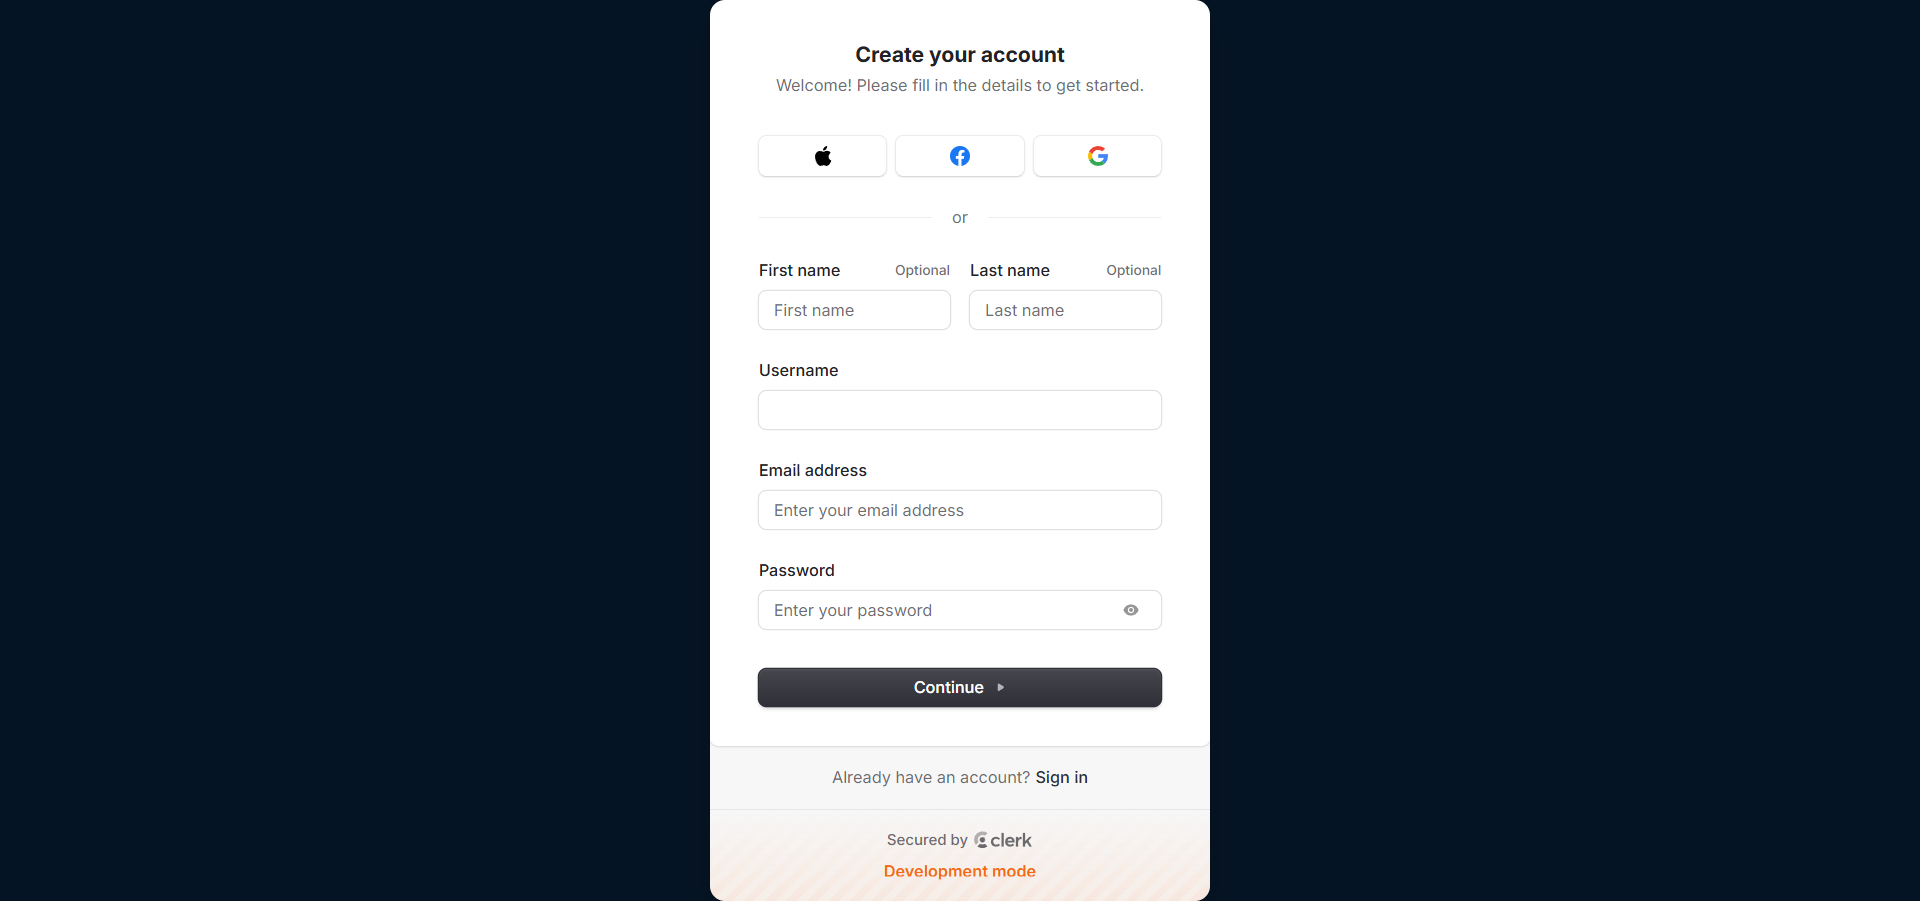
\includegraphics[width=0.45\textwidth, keepaspectratio]{Figures/22.png}
    }{}
    \hfill
    \IfFileExists{Figures/3.png}{
        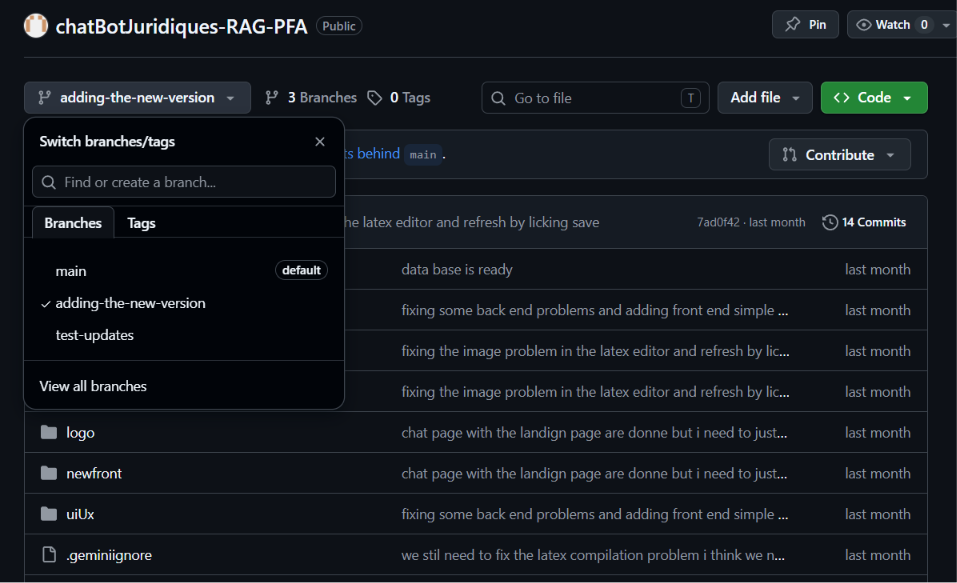
\includegraphics[width=0.45\textwidth, keepaspectratio]{Figures/3.png}
    }{}
    \caption{Clerk Authentication Portals: Account Creation (Left) and Sign-In (Right).}
    \label{fig:demo_auth}
\end{figure}

\subsection{Interactive Consultation and RAG Navigation}
Post-authentication, the user transitions to the AI Chat Interface, featuring a clean, minimalist dashboard. The left sidebar presents their chat history, intelligently categorized into "Pinned" and "Recent" sessions. A contextual menu (accessible via a three-dot icon) permits users to rename sessions inline, pin critical threads to the top, or delete them entirely. In the primary chat window, users can initialize a "New Chat" for fresh consultations or utilize the semantic search bar to rapidly retrieve previous conversations based on specific keywords.

\IfFileExists{Figures/7.png}{
    \begin{figure}[H]
        \centering
        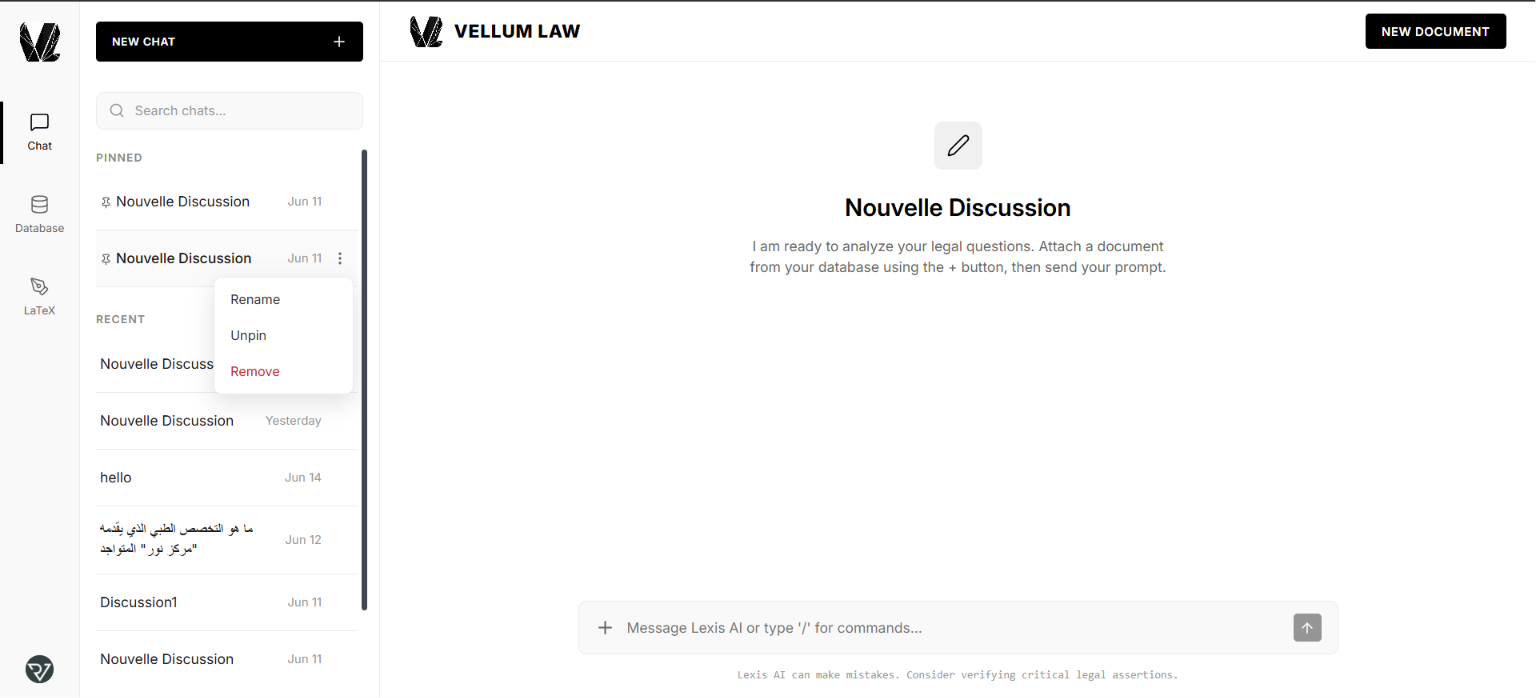
\includegraphics[width=0.85\textwidth, keepaspectratio]{Figures/7.png}
        \caption{Initial Chat Dashboard Layout and History Navigation Utilities.}
        \label{fig:demo_chat_init}
    \end{figure}
}{}

During interactions, the user inputs complex legal queries into the text area. The AI's response is dynamically rendered through a custom Markdown interpretation layer, ensuring that structured tables, bold emphasis, and bidirectional text (automatically aligning Arabic Right-To-Left and French Left-To-Right) are displayed impeccably. Furthermore, should the AI rely on general pre-trained knowledge due to insufficient retrieved context, a graceful fallback disclaimer is prominently displayed at the bottom of the response, maintaining absolute transparency.

\begin{figure}[H]
    \centering
    \IfFileExists{Figures/4.png}{
        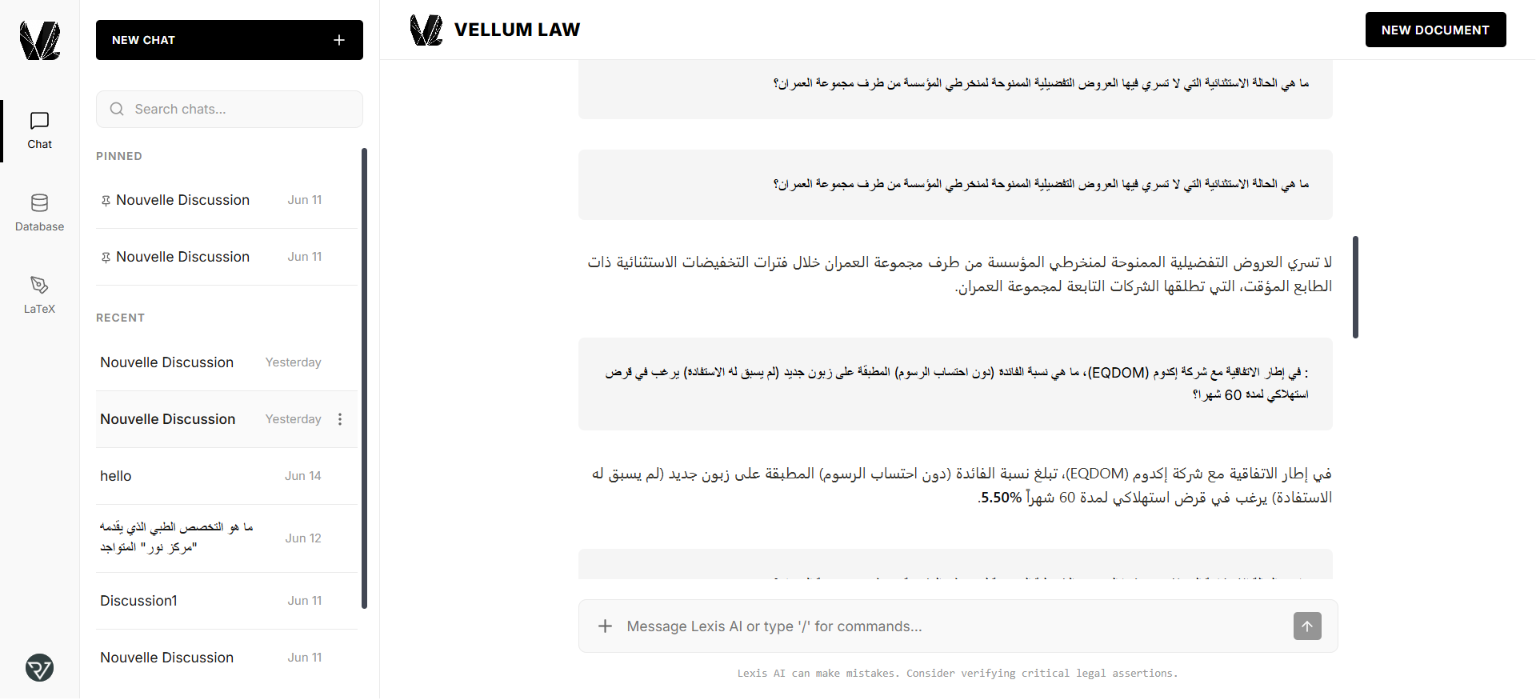
\includegraphics[width=0.8\textwidth, keepaspectratio]{Figures/4.png}\\[0.5cm]
    }{}
    \IfFileExists{Figures/5.png}{
        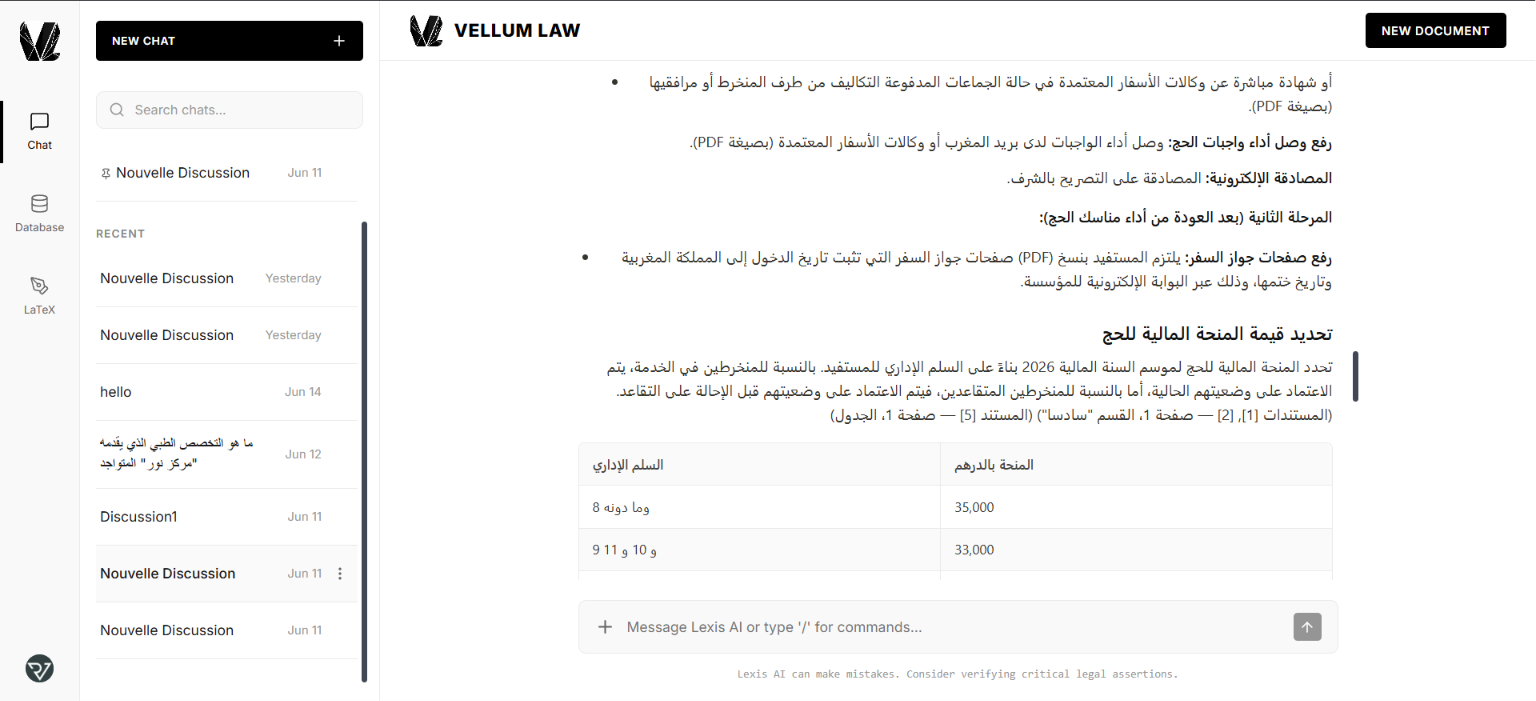
\includegraphics[width=0.8\textwidth, keepaspectratio]{Figures/5.png}
    }{}
    \caption{Active RAG Chat Sessions Rendering Bilingual Markdown and Formatted Tables.}
    \label{fig:demo_chat_active}
\end{figure}

To expand the scope of the consultation, the user can click the "+" icon within the chat input to attach live documents (PDFs or images) directly from their database, seamlessly triggering the system's Live File Bypass multimodal pipeline.

\IfFileExists{Figures/6.png}{
    \begin{figure}[H]
        \centering
        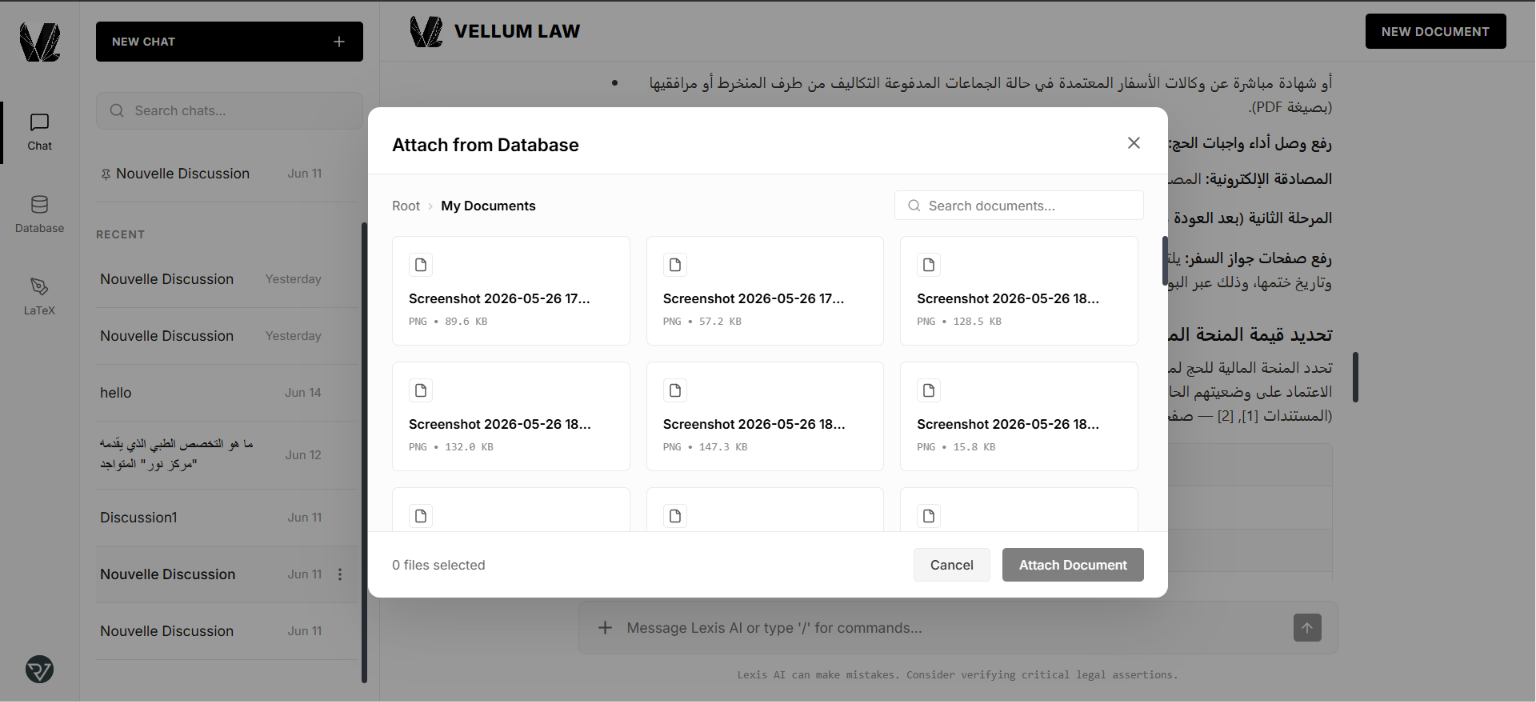
\includegraphics[width=0.85\textwidth, keepaspectratio]{Figures/6.png}
        \caption{Live File Attachment Modal Triggered from the Chat Input.}
        \label{fig:demo_chat_modal}
    \end{figure}
}{}

\subsection{Document Management System (DMS) Overview}
The Document Management System (DMS) acts as a secure, interactive vault for the user's legal files. Users can invoke a custom modal via the "New Folder" button to create virtual directories. An interactive breadcrumb navigation system (e.g., \texttt{Root > My Documents}) facilitates deep traversal into the folder hierarchy or rapid returns to the root directory. The interface effortlessly toggles between Grid and List view modes, and supports bulk drag-and-drop operations, directly persisting files to both local storage and the PostgreSQL database.

\IfFileExists{Figures/8.png}{
    \begin{figure}[H]
        \centering
        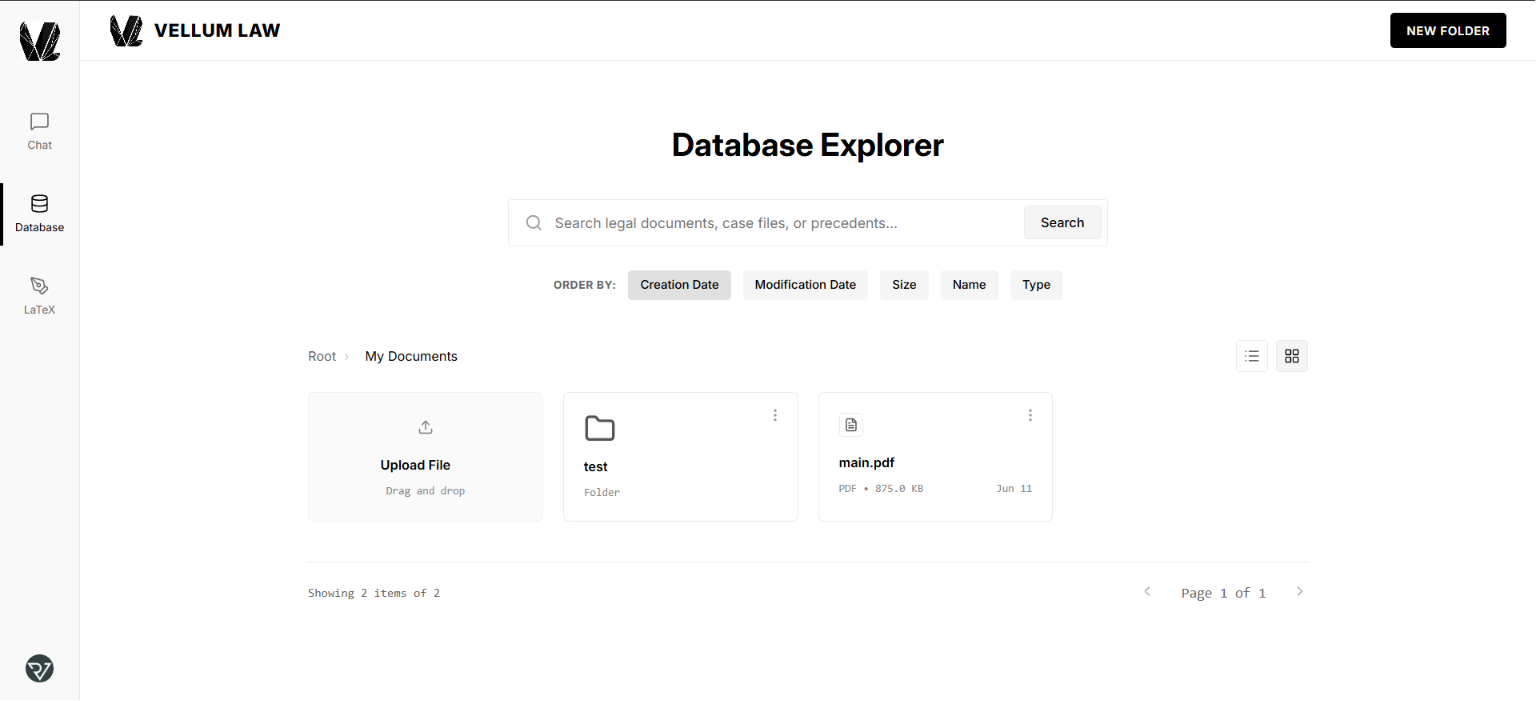
\includegraphics[width=0.85\textwidth, keepaspectratio]{Figures/8.png}
        \caption{DMS Interface Displaying the Virtual Folder Creation Modal.}
        \label{fig:demo_dms_root}
    \end{figure}
}{}

To manage large datasets efficiently, the DMS features an "Order By" dropdown menu, allowing dynamic sorting by Creation Date, Modification Date, Size, Name, or Type. Clicking the "Rename" option instantly transforms the asset's title into an inline text input, bypassing intrusive browser pop-ups for a superior user experience. Dynamic pagination controls at the bottom of the page ensure smooth navigation through extensive libraries without compromising UI integrity.

\IfFileExists{Figures/9.png}{
    \begin{figure}[H]
        \centering
        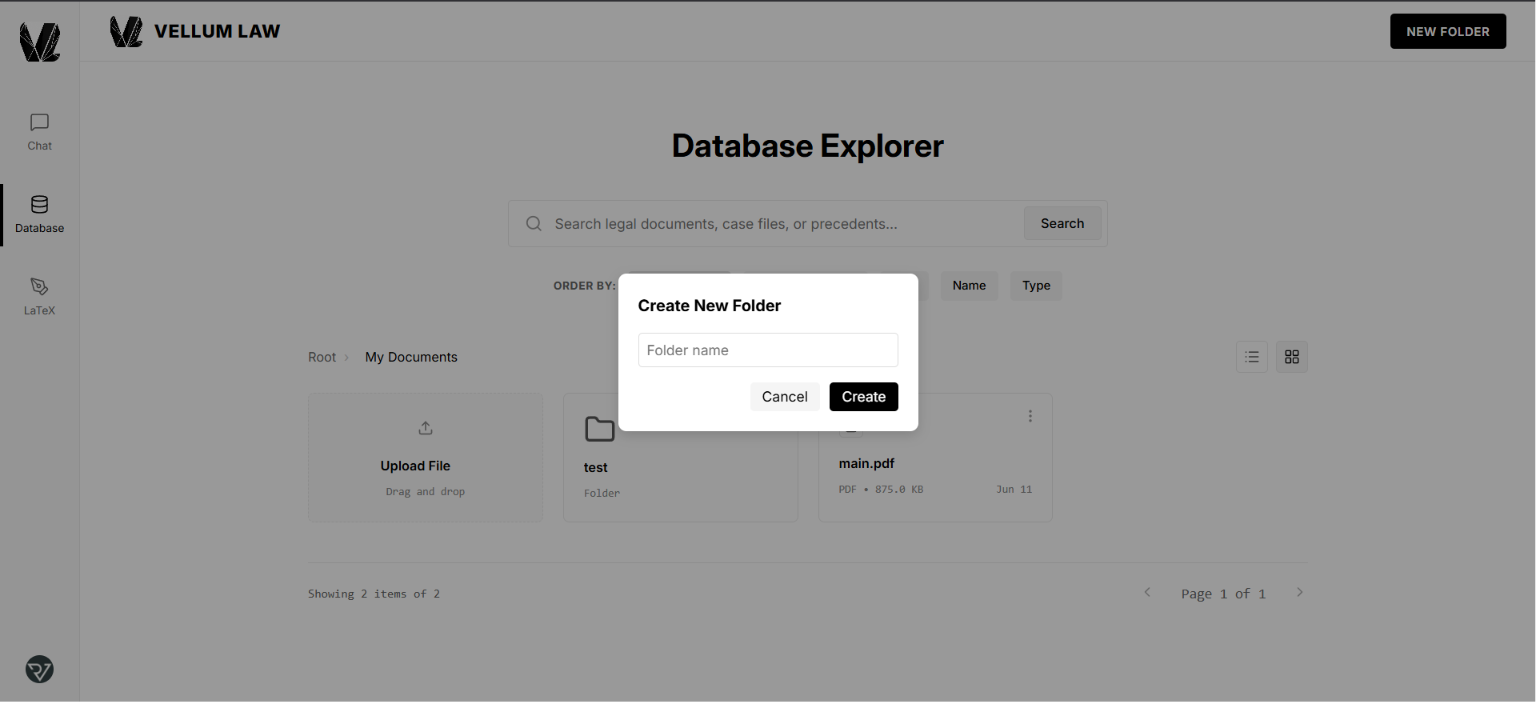
\includegraphics[width=0.85\textwidth, keepaspectratio]{Figures/9.png}
        \caption{DMS Explorer Highlighting Dynamic Sorting and Pagination Controls.}
        \label{fig:demo_dms_sort}
    \end{figure}
}{}

\subsection{LaTeX Legal Editor and AI Assistant}
The Legal Template Editor workspace presents a highly productive split-screen layout. The left navigation panel organizes \LaTeX\ projects into Pinned and Recent categories, maintaining UX consistency with the Chat Interface.

\IfFileExists{Figures/10.png}{
    \begin{figure}[H]
        \centering
        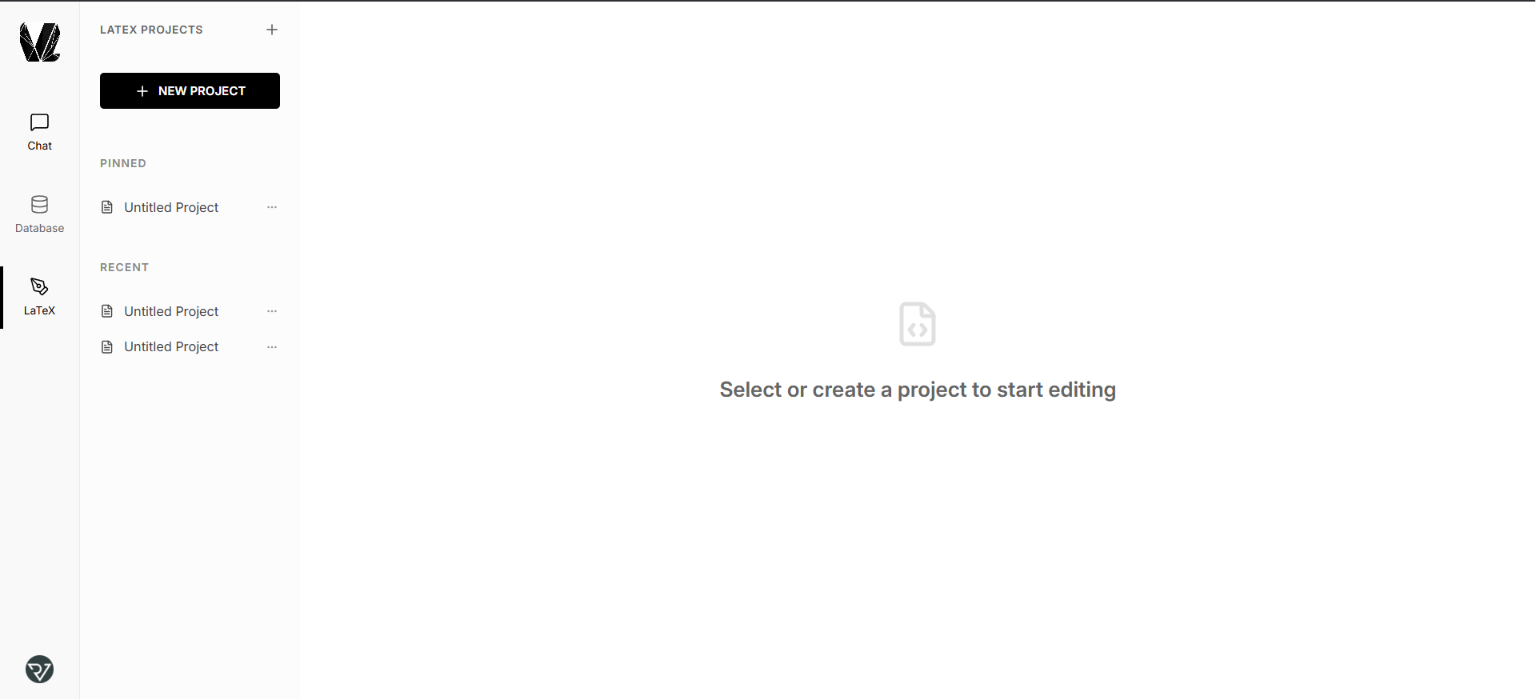
\includegraphics[width=0.85\textwidth, keepaspectratio]{Figures/10.png}
        \caption{Initial State of the LaTeX Workspace and Project Explorer.}
        \label{fig:demo_latex_init}
    \end{figure}
}{}

The central workspace features a robust code editor juxtaposed with a Live PDF Viewer. Users can manually edit their \LaTeX\ code and initiate a "Compile" command to render a professional PDF document instantaneously. The backend routing engine intelligently evaluates the payload, directing text-only compilations to the ultra-fast LaTeXLite cloud API, or utilizing a local \texttt{pdflatex} engine if complex image assets are detected.

\begin{figure}[H]
    \centering
    \IfFileExists{Figures/11.png}{
        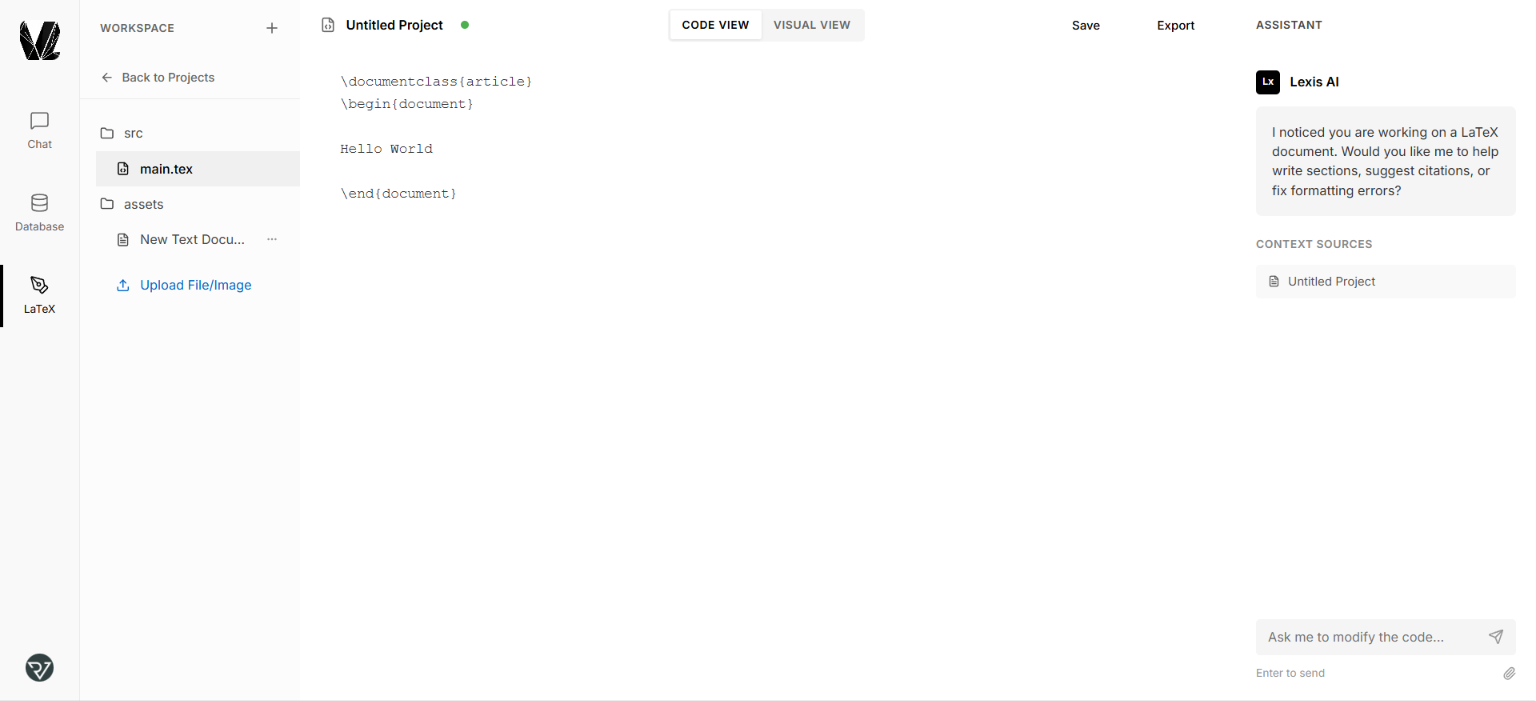
\includegraphics[width=0.8\textwidth, keepaspectratio]{Figures/11.png}\\[0.5cm]
    }{}
    \IfFileExists{Figures/12.png}{
        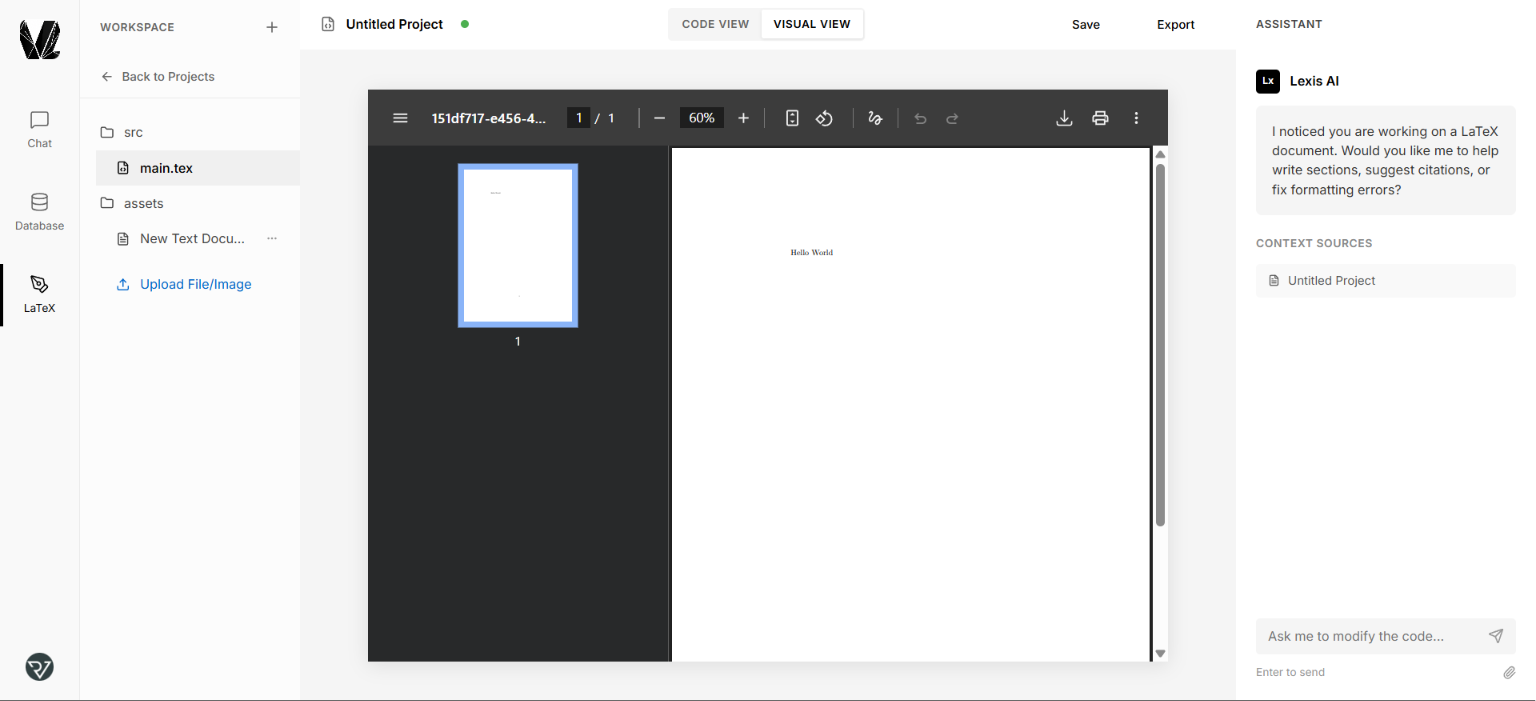
\includegraphics[width=0.8\textwidth, keepaspectratio]{Figures/12.png}
    }{}
    \caption{Split-Screen Editor Toggling Between Raw Code View (Top) and Visual PDF Render (Bottom).}
    \label{fig:demo_editor_views}
\end{figure}

The rightmost panel houses a dedicated AI Assistant. Users can command the AI to modify the active document, with the backend automatically injecting the project's assets as context.

\IfFileExists{Figures/13.png}{
    \begin{figure}[H]
        \centering
        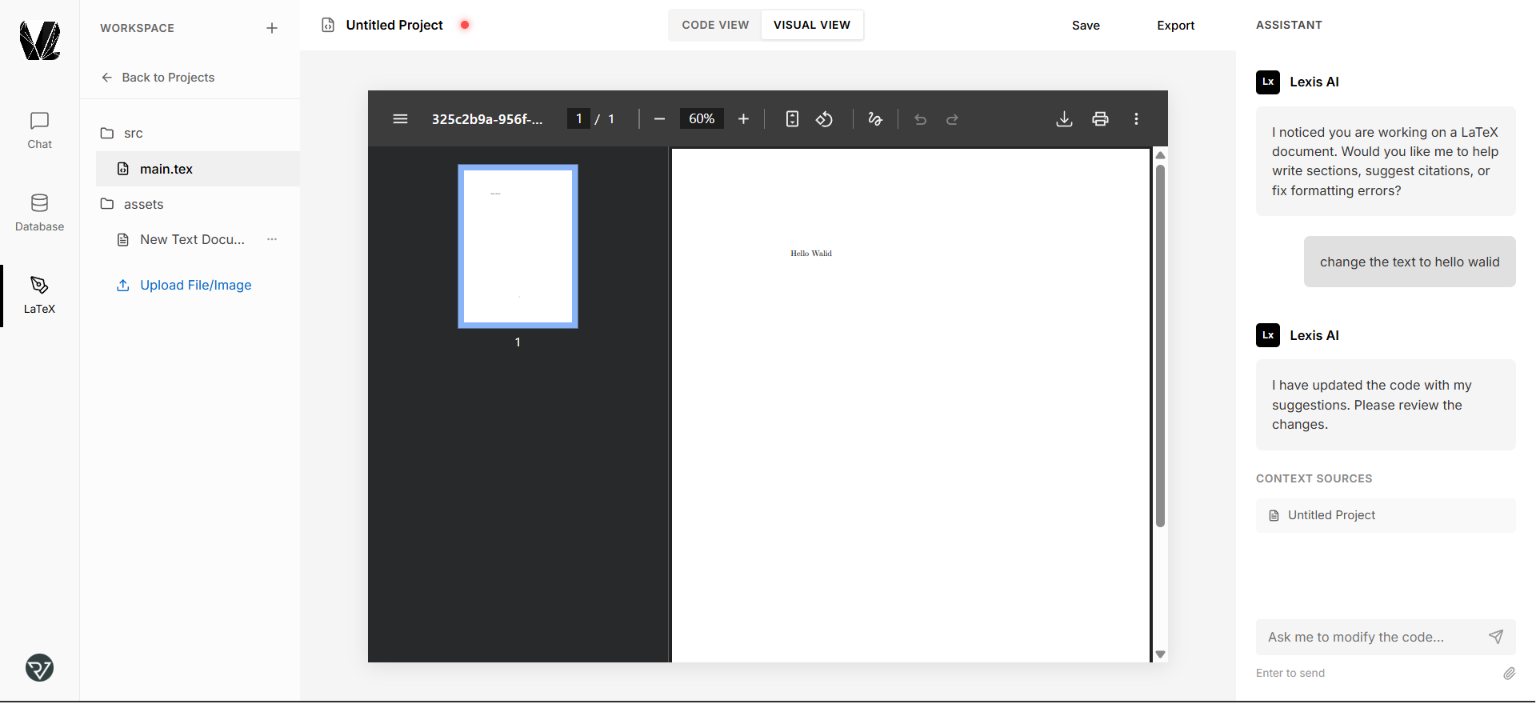
\includegraphics[width=0.85\textwidth, keepaspectratio]{Figures/13.png}
        \caption{AI Assistant Processing Document Context to Suggest Direct Edits.}
        \label{fig:demo_editor_ai}
    \end{figure}
}{}

Crucially, the interface supports specialized slash-commands (e.g., "\texttt{/template NDA}"). This action triggers the AI to query the backend JSON registry, retrieve the requested legal template, intelligently populate placeholders based on the user's prompt, and autonomously inject the flawlessly formatted \LaTeX\ code directly into the editor.

\IfFileExists{Figures/14.png}{
    \begin{figure}[H]
        \centering
        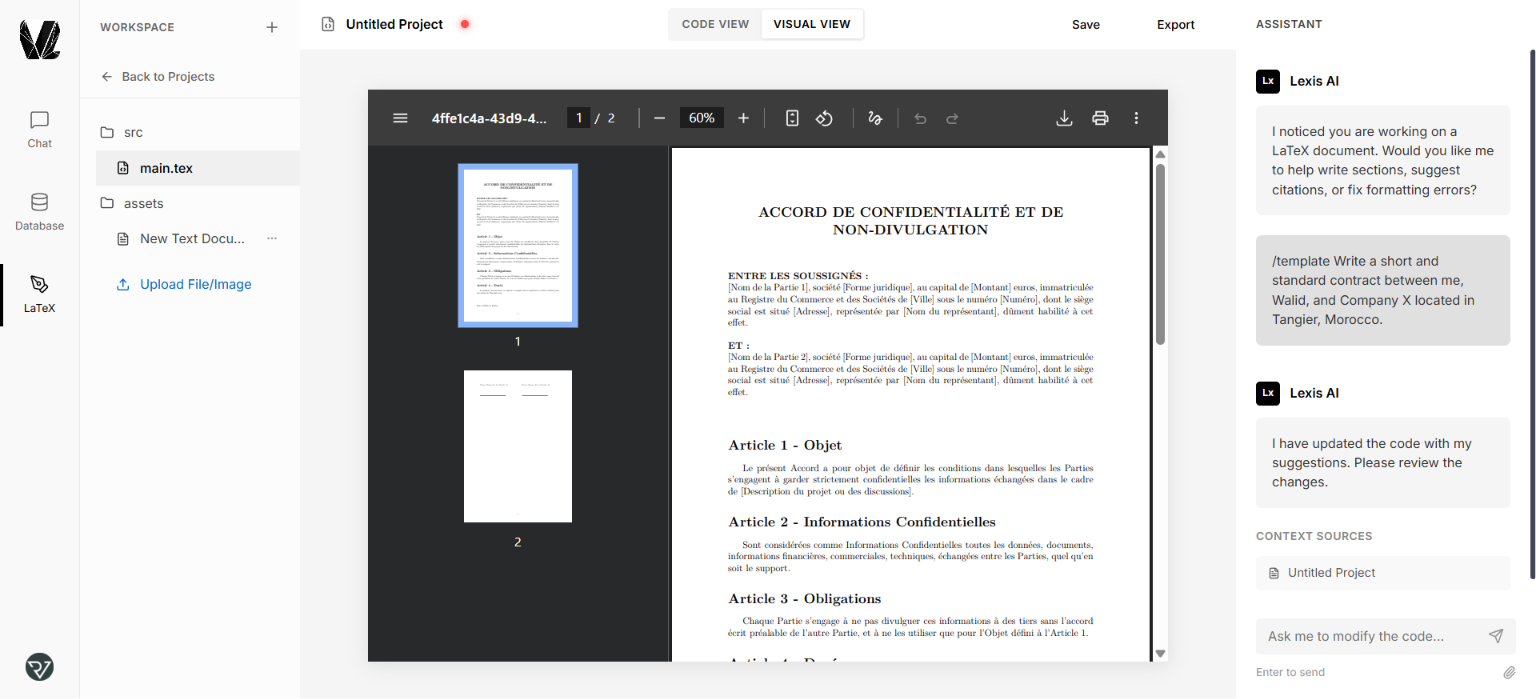
\includegraphics[width=0.85\textwidth, keepaspectratio]{Figures/14.png}
        \caption{Execution of the \texttt{/template} Slash-Command Autonomously Generating a Contract.}
        \label{fig:demo_editor_template}
    \end{figure}
}{}

\newpage
\section{Technical and Algorithmic Evaluation}
To validate the platform's readiness for production deployment, a rigorous technical evaluation was conducted on our high-concurrency architecture, assessing core processing speeds and RAG intelligence validation loops.

\subsection{Backend API Performance and Latency Analysis}
The backend application layer underwent comprehensive benchmarking under simulated heavy-load environments to confirm that the asynchronous FastAPI gateway can reliably route traffic without deadlocking the event pool loop.

\begin{itemize}
    \item \textbf{Endpoint Latency Performance:} Network latency and database query routing durations were audited across vital processing actions. The baseline results under concurrent load testing are documented below:
\end{itemize}

\begin{table}[H]
\centering
\caption{FastAPI Endpoint Baseline Latency Metrics.}
\label{tab:latency_metrics}
\renewcommand{\arraystretch}{1.3} % Enhance row spacing for professional look
\begin{tabular}{@{}l c c c@{}}
\toprule
\textbf{API Endpoint Route} & \textbf{HTTP Method} & \textbf{Simulated Load Condition} & \textbf{Average Latency} \\ 
\midrule
\texttt{/api/v1/auth/session}  & GET  & 100 Concurrent Connections & 142 ms  \\ 
\texttt{/api/v1/database/upload} & POST & 50 MB Multi-page Document  & 2.1 s \\ 
\texttt{/api/v1/editor/compile}  & POST & 12-Page Complex TeX Project & 1.3 s \\ 
\bottomrule
\end{tabular}
\end{table}

\begin{itemize}
    \item \textbf{Tenant Isolation \& Resource Scaling:} Continuous evaluation of the persistence layer confirmed that row-level security (RLS) policies and dynamic database pool limits scale seamlessly, effectively isolating background file processing tasks without exhausting main server resources.
\end{itemize}

\subsection{RAG Pipeline Accuracy and Retrieval Metrics}
The retrieval system was meticulously audited under concrete Moroccan legal scenarios to verify that the multi-query decomposition and cross-encoder reranking loops effectively neutralize hallucinations.

\begin{itemize}
    \item \textbf{Retrieval Index Performance:} The vector engine's ability to search dense arrays using multilingual semantic matches was evaluated based on Cosine Similarity:
    $$ \text{Similarity}(A, B) = \frac{A \cdot B}{\|A\| \|B\|} $$
    The cross-encoder reranking layer successfully isolates and elevates the top 5 absolute most accurate legal contexts from the broad initial retrieval.
    
    \item \textbf{Core Intelligence Metric Evaluation:} The grounded generation pipeline was systematically evaluated against three cardinal production metrics:
    \begin{enumerate}
        \item \textbf{Faithfulness:} Verifies that all generated assertions depend strictly and exclusively on the retrieved legal contexts, mathematically eliminating hallucination risks.
        \item \textbf{Answer Relevance:} Confirms that the generative output directly and efficiently addresses the core legal intent of the original user prompt.
        \item \textbf{Context Recall:} Ensures the vector database retrieval loop successfully surfaces all mandatory legal articles required to form a complete and definitive answer.
    \end{enumerate}
\end{itemize}

\IfFileExists{Figures/rag_eval_chart.png}{
    \begin{figure}[H]
        \centering
        \includegraphics[width=0.75\textwidth, keepaspectratio]{Figures/rag_eval_chart.png}
        \caption{Algorithmic Accuracy Scores across RAG Pipeline Phases.}
        \label{fig:rag_eval_metrics}
    \end{figure}
}{}

\newpage
\section*{Conclusion}
The experimental results definitively demonstrate that the implemented architecture delivers the high-speed execution and precision metrics required for an enterprise-grade Moroccan LegalTech platform. By leveraging non-blocking asynchronous routing strategies alongside a highly refined, multi-stage retrieval pipeline, the platform manages compute-heavy AI operations with exceptional efficiency. This robust structure securely processes complex legal queries while guaranteeing absolute data isolation and negligible response latencies.

\chapter*{General Conclusion and Perspectives}

\addcontentsline{toc}{chapter}{General Conclusion and Perspectives}

\label{chap:General_Conclusion} 

The conceptualization, design, and deployment of this LegalTech platform represent a significant milestone in modernizing administrative and legal workflows within the Moroccan context. By integrating state-of-the-art artificial intelligence—specifically through a highly optimized Retrieval-Augmented Generation (RAG) architecture—this project successfully bridges the gap between traditional legal research methodologies and next-generation, automated semantic analysis. 

Throughout the development lifecycle, we systematically addressed several critical bottlenecks prevalent in the legal sector. By employing advanced Vision-Language Models (GPT-4o Vision), we overcame the persistent challenges of ingesting unstructured, image-based Moroccan legal documents. Our highly structured prompt engineering and custom XML chunking logic guaranteed that complex matrices, legal tables, and textual nuances were flawlessly indexed without losing semantic fidelity. Furthermore, by coupling a robust vector database (ChromaDB) with a multi-stage retrieval loop—incorporating cross-encoder reranking and dynamic query decomposition—we effectively neutralized the risk of AI hallucination, ensuring that all generated responses are strictly anchored in verifiable Moroccan legal jurisprudence.

Beyond the algorithmic achievements in the backend, the platform delivers a cohesive, enterprise-grade user experience. The integration of a secure Document Management System (DMS), a multimodal conversational interface, and an autonomous \LaTeX\ drafting workspace empowers legal professionals to perform end-to-end case management within a single, highly performant ecosystem. The architectural decisions—ranging from the asynchronous FastAPI orchestration to the reactive, decoupled React frontend—ensure that the platform remains highly scalable, exceptionally fast, and rigorously secure.

\section*{Future Perspectives}

While the current iteration of the platform meets all predefined operational and academic objectives, the architecture was intentionally designed to support future extensibility. Potential avenues for future development include:

\begin{itemize}
    \item \textbf{Integration of Agentic Workflows:} Evolving the current RAG pipeline into an autonomous, multi-agent framework capable of executing complex, multi-step legal research across external governmental databases in real-time.
    \item \textbf{Predictive Legal Analytics:} Leveraging historical case law and quantitative litigation data to predict case outcomes, estimate legal costs, and recommend optimal negotiation strategies based on statistical probabilities.
    \item \textbf{Expanded Multilingual Capabilities:} While the system currently excels in formal Arabic and French, extending the semantic engine to support local dialects (Darija) could further democratize access to legal consultations for the general public.
    \item \textbf{Blockchain Integration for Document Verification:} Implementing immutable, cryptographic ledger technologies to digitally sign, notarize, and verify the authenticity of contracts and legal documents generated within the \LaTeX\ workspace.
\end{itemize}

Ultimately, this project stands as a testament to the transformative potential of Artificial Intelligence in the legal domain. It demonstrates that with meticulous architectural planning, rigorous data engineering, and a focus on user-centric design, it is entirely possible to construct an intelligent system capable of navigating the intricate, highly consequential realm of law.

\appendix


\input{Endmatter/Glossary}

\input{Endmatter/Acronyms}

\input{Endmatter/ComplementaryCodes}

\begin{thebibliography}{99}
\addcontentsline{toc}{chapter}{Bibliography}


\bibitem{ref1}
Author name, Book name.

\bibitem{ref2}
\emph{Title 1},
\href{https://www.overleaf.com/learn/latex/Bibliography_management_with_bibtex}{\textbf{Title 2}}

 %the link is a documentation of the basic bibliography method (that    I'm using here) + bibTex which is more advanced, read it well and decide which one works best for you.



\end{thebibliography}

\end{document}